
\documentclass{article}
\usepackage[utf8]{inputenc}
\usepackage[titletoc, title]{appendix}
\usepackage{geometry}
\geometry{
 a4paper,
 left=27mm,
 top=30mm,
 }
\usepackage{ amssymb }
\usepackage{graphicx} % Required for the inclusion of images
\usepackage{caption}
\usepackage{subcaption}
\usepackage{amsmath} % Required for some math elements
\usepackage[labelfont=bf]{caption}



\usepackage{hyperref}
\usepackage{float}

%\for code
\usepackage{listings}
\usepackage{xcolor}

\definecolor{codegreen}{rgb}{0,0.6,0}
\definecolor{codegray}{rgb}{0.5,0.5,0.5}
\definecolor{codepurple}{rgb}{0.58,0,0.82}
\definecolor{backcolour}{rgb}{0.95,0.95,0.92}

\lstdefinestyle{mystyle}{
    backgroundcolor=\color{backcolour},
    commentstyle=\color{codegreen},
    keywordstyle=\color{magenta},
    numberstyle=\tiny\color{codegray},
    stringstyle=\color{codepurple},
    basicstyle=\ttfamily\footnotesize,
    breakatwhitespace=false,
    breaklines=true,
    captionpos=b,
    keepspaces=true,
    numbers=left,
    numbersep=5pt,
    showspaces=false,
    showstringspaces=false,
    showtabs=false,
    tabsize=2
}

\lstset{style=mystyle}





%\setlength\parindent{0pt} % Removes all indentation from paragraphs
\usepackage{authblk}
\usepackage{wrapfig}
%\renewcommand{\labelenumi}{\alph{enumi}.} % Make numbering in the enumerate environment by letter rather than number (e.g. section 6)
\usepackage[font={small}]{caption}
%\newcommand*\diff{\mathop{}\!\mathrm{d}}
\usepackage{tikz}
\usepackage{placeins}



%----------------------------------------------------------------------------------------
%	DOCUMENT INFORMATION
%----------------------------------------------------------------------------------------

\title{Networks} % Title

\author{Florian \textsc{Leprévost}} % Author name

\date{\today} % Date for the report

\begin{document}
\maketitle % Insert the title, author and date

\noindent Supervisor: Manuel Beiran % Instructor/supervisor
\tableofcontents

\begin{center}
\begin{tabular}{l r}

\end{tabular}
\end{center}

%----------------------------------------------------------------------------------------
%	SECTION 0
%----------------------------------------------------------------------------------------

\section{Introduction}\label{introduction}

\indent\indent One of the most exciting aspect of Computational neuroscience, is the possibility to simulate neuronal networks. For instance, one can assess the implementational plausibility of computational acount of cognitive processes. Outside of neuroscience, artificial neural networks are also used to perform some tasks computers are usually not very good at: classification tasks, face and speech recognition, game playing, etc. (\href{https://en.wikipedia.org/wiki/Artificial_neural_network}{wikipedia}).\\

\indent Contrary to those latter applications, neural networks built in neuroscience try to take into account the biophysical properties of neurons as much as possible. However, some aspects can be simplified without altering too much the descriptive properties of the system. Moreover, we can use the dynamical systems' approach to better study the behavior of those networks for given parameters.\\
%----------------------------------------------------------------------------------------
%	SECTION 1
%----------------------------------------------------------------------------------------

\section{Neuron with autapse}\label{autapse}
\indent\indent To simplify the network models, we can use a differential equation describing neurons' firing rate (spike per second) rather than simulating their membrane voltage and spiking mechanism. For instance, we can consider the following extra-simple network of a neuron with a synaptic connection to itself (an \textit{autapse}). Let $x$ be the neuron's firing rate, $w$ the strength of the synaptic weight, $I$ some constant external input, and $f$ an activation function:

\begin{equation}\label{eq:1}
  \dot{x}(t) = -x(t) + f(wx(t) +I)
\end{equation}

Consequently, the system (\ref{eq:1})'s dynamics can be approximated with the Euler method as follows:

\begin{align*}\label{eq:2}
  {x}(t+1) &= x(t) + \dot{x}(t)\delta t\\
            &= x(t) + (-x(t) + f(wx(t) +I))\delta t
\end{align*}

When looking at spiking neurons, the activation (or input-output) function is a `threshold' function, usually non linear or sigmoidal, that determines the input value necessary to trigger an action potential (or a spike). Considering the system we have, the activation function determines here rather the input necessary in order to trigger auto-sustained activity in this neuron. Let's consider the following activation function $f$, using the hyperbolic tangent to create a sigmoid (Figure \ref{fig:fig1}):

\begin{equation}
  f(s) = 50 (1 + tanh(s))
\end{equation}

\begin{figure}[H]
\centering
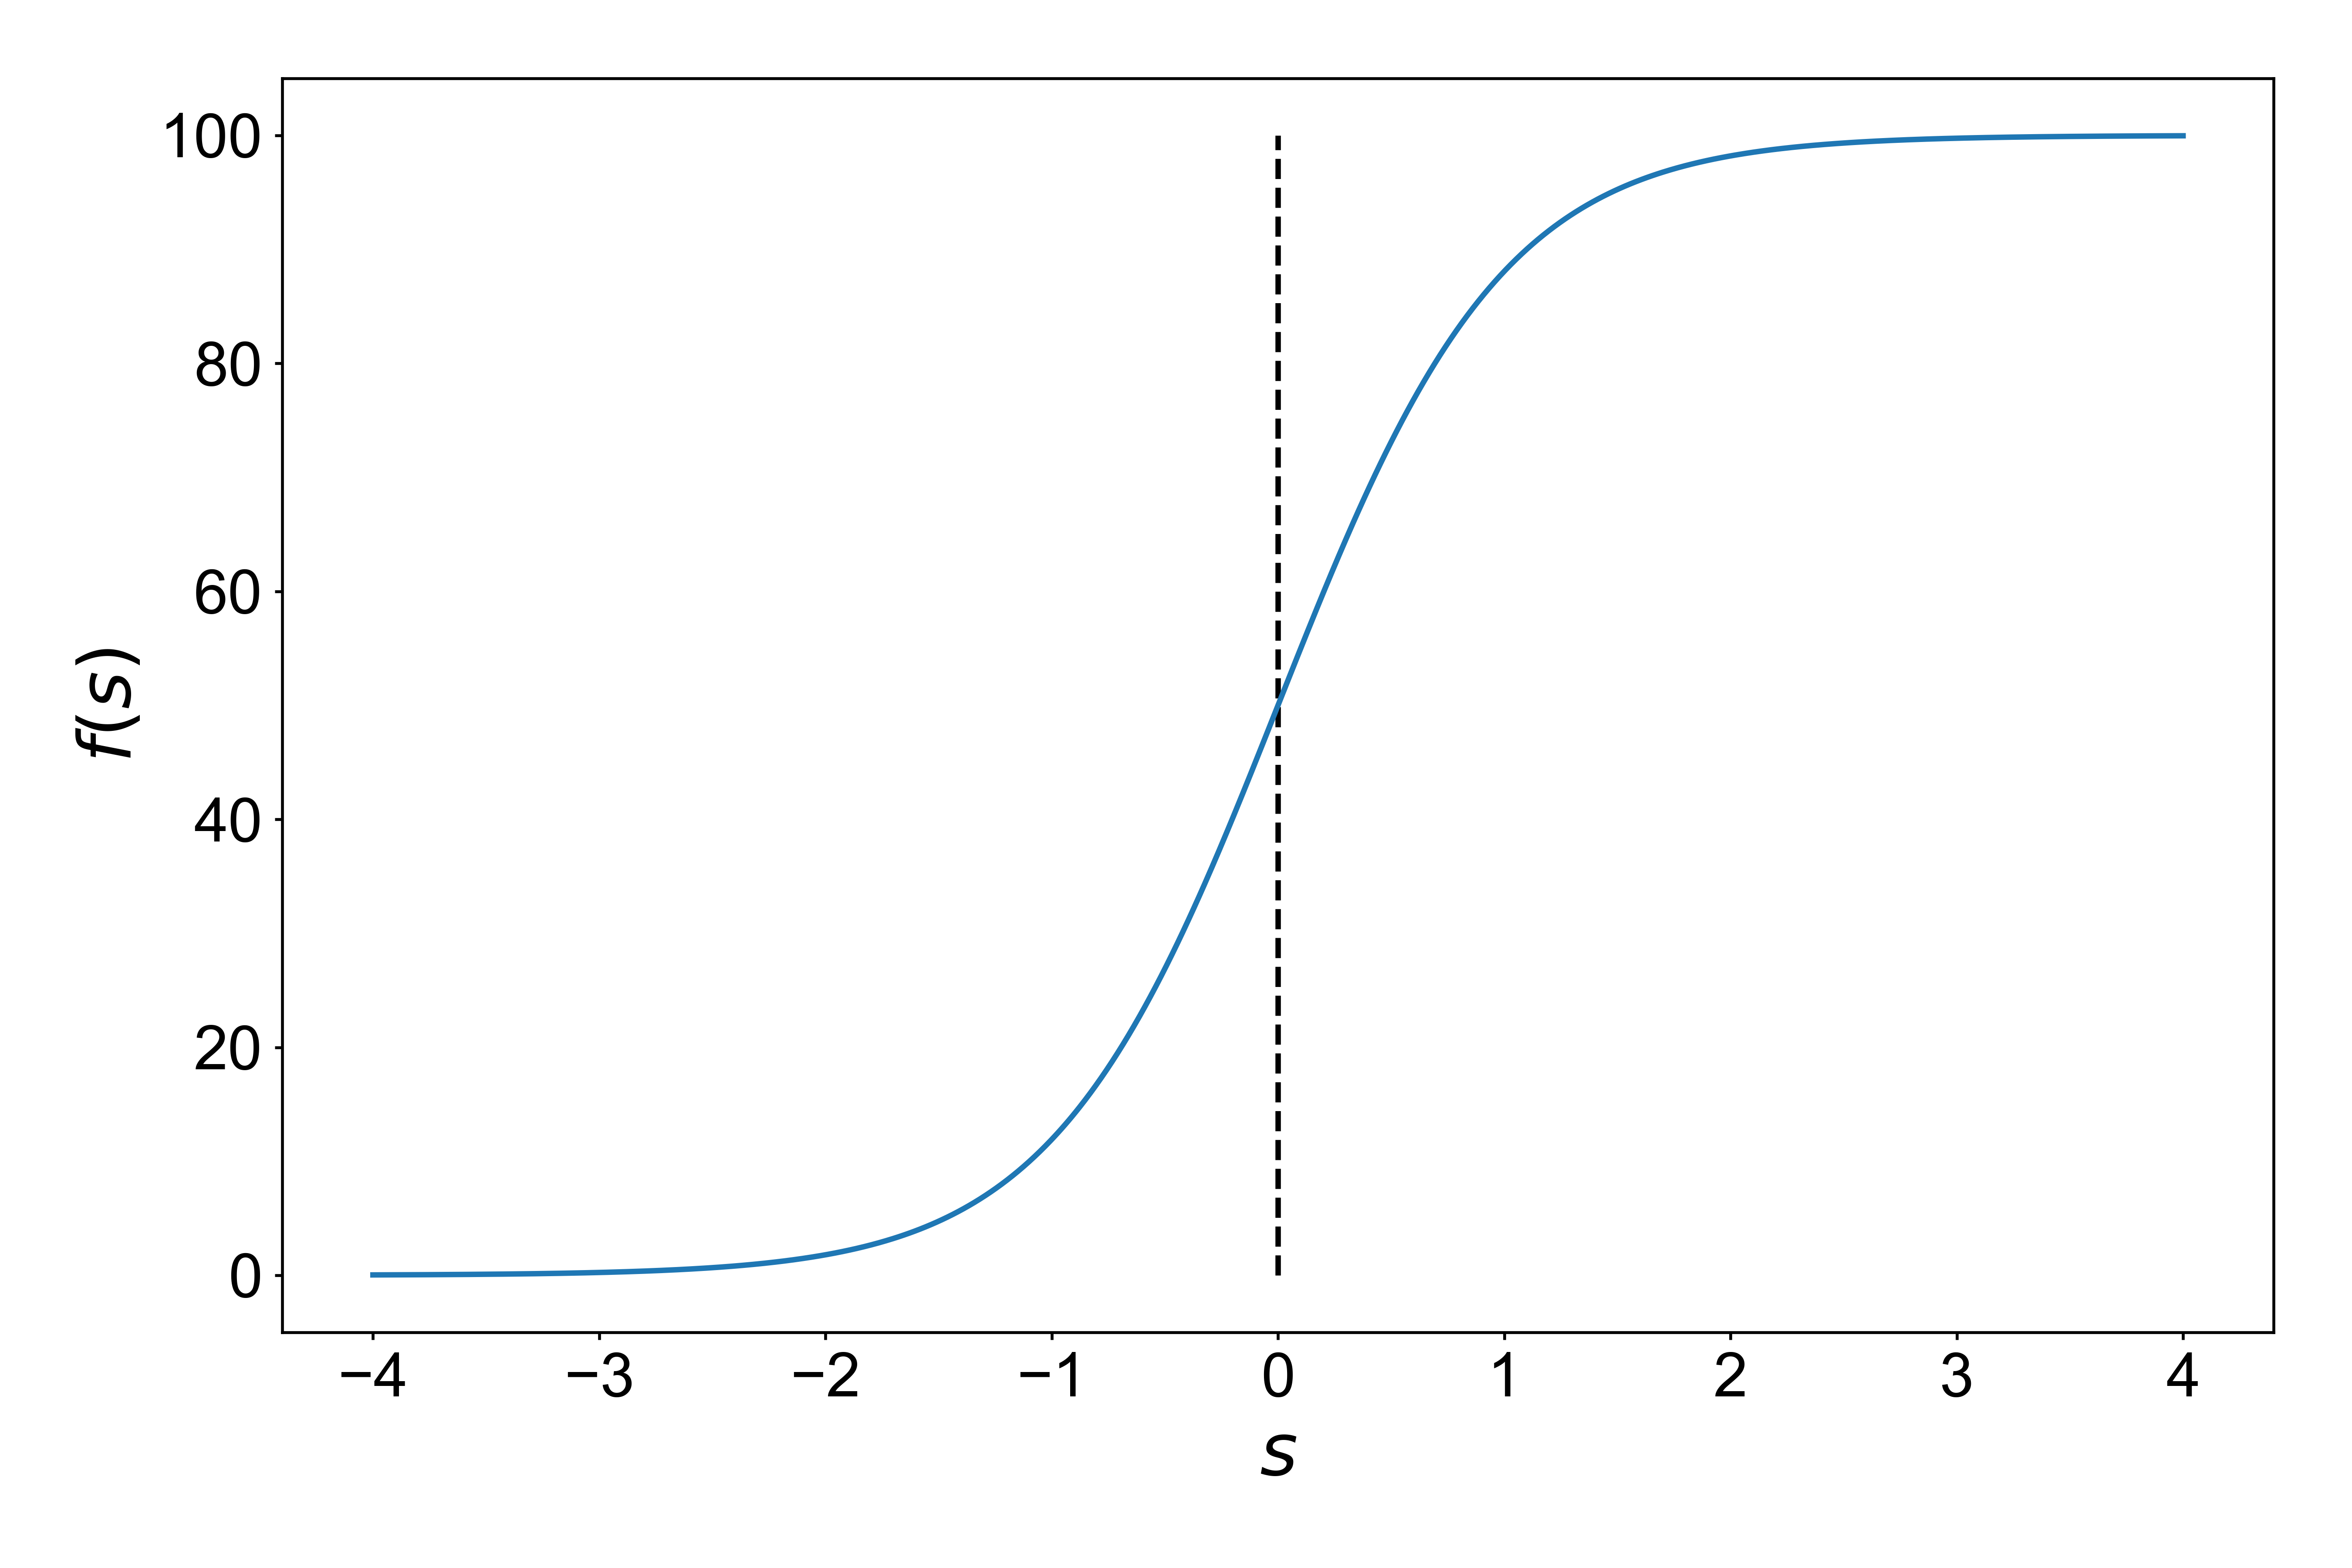
\includegraphics[width=.8\linewidth]{exercice5fig1.png}
\caption[spt]{Activation function $f(s)$'s behavior for values of $s$ near 0.}\label{fig:fig1}
\end{figure}

Dynamical system's approach to differential equations allows to visualize which are the fixed points in the system, i.e. the values of $x$ for which $\dot{x}=0$. When the system reaches such a point, its value (here the neuron's firing rate) is going to remain constant. Moreover, depending on the sign of the derivative around those point, the system is going to be attracted to them or repelled from them.\\

Figure \ref{fig:fig2} shows $\dot{x}(t)$ as a function of $x(t)$, for a system with a  weight $w=0.04$, a time step $\delta t = 0.1$, and a constant inhibitory current $I=-2$ . If for a given t,  $\dot{x}(t)$ is negative, $x(t)$ is going to decrease progressively to the next inferior fixed point. Similarly, if $\dot{x}(t)$ is positive, the system is going to increase to the next superior fixed point. This is why some fixed points of the systems are actually attractors ($x$ tends towards them when it has close value) and some repellors ($x$ tends away from them when it has close value).

\begin{figure}[H]
\centering
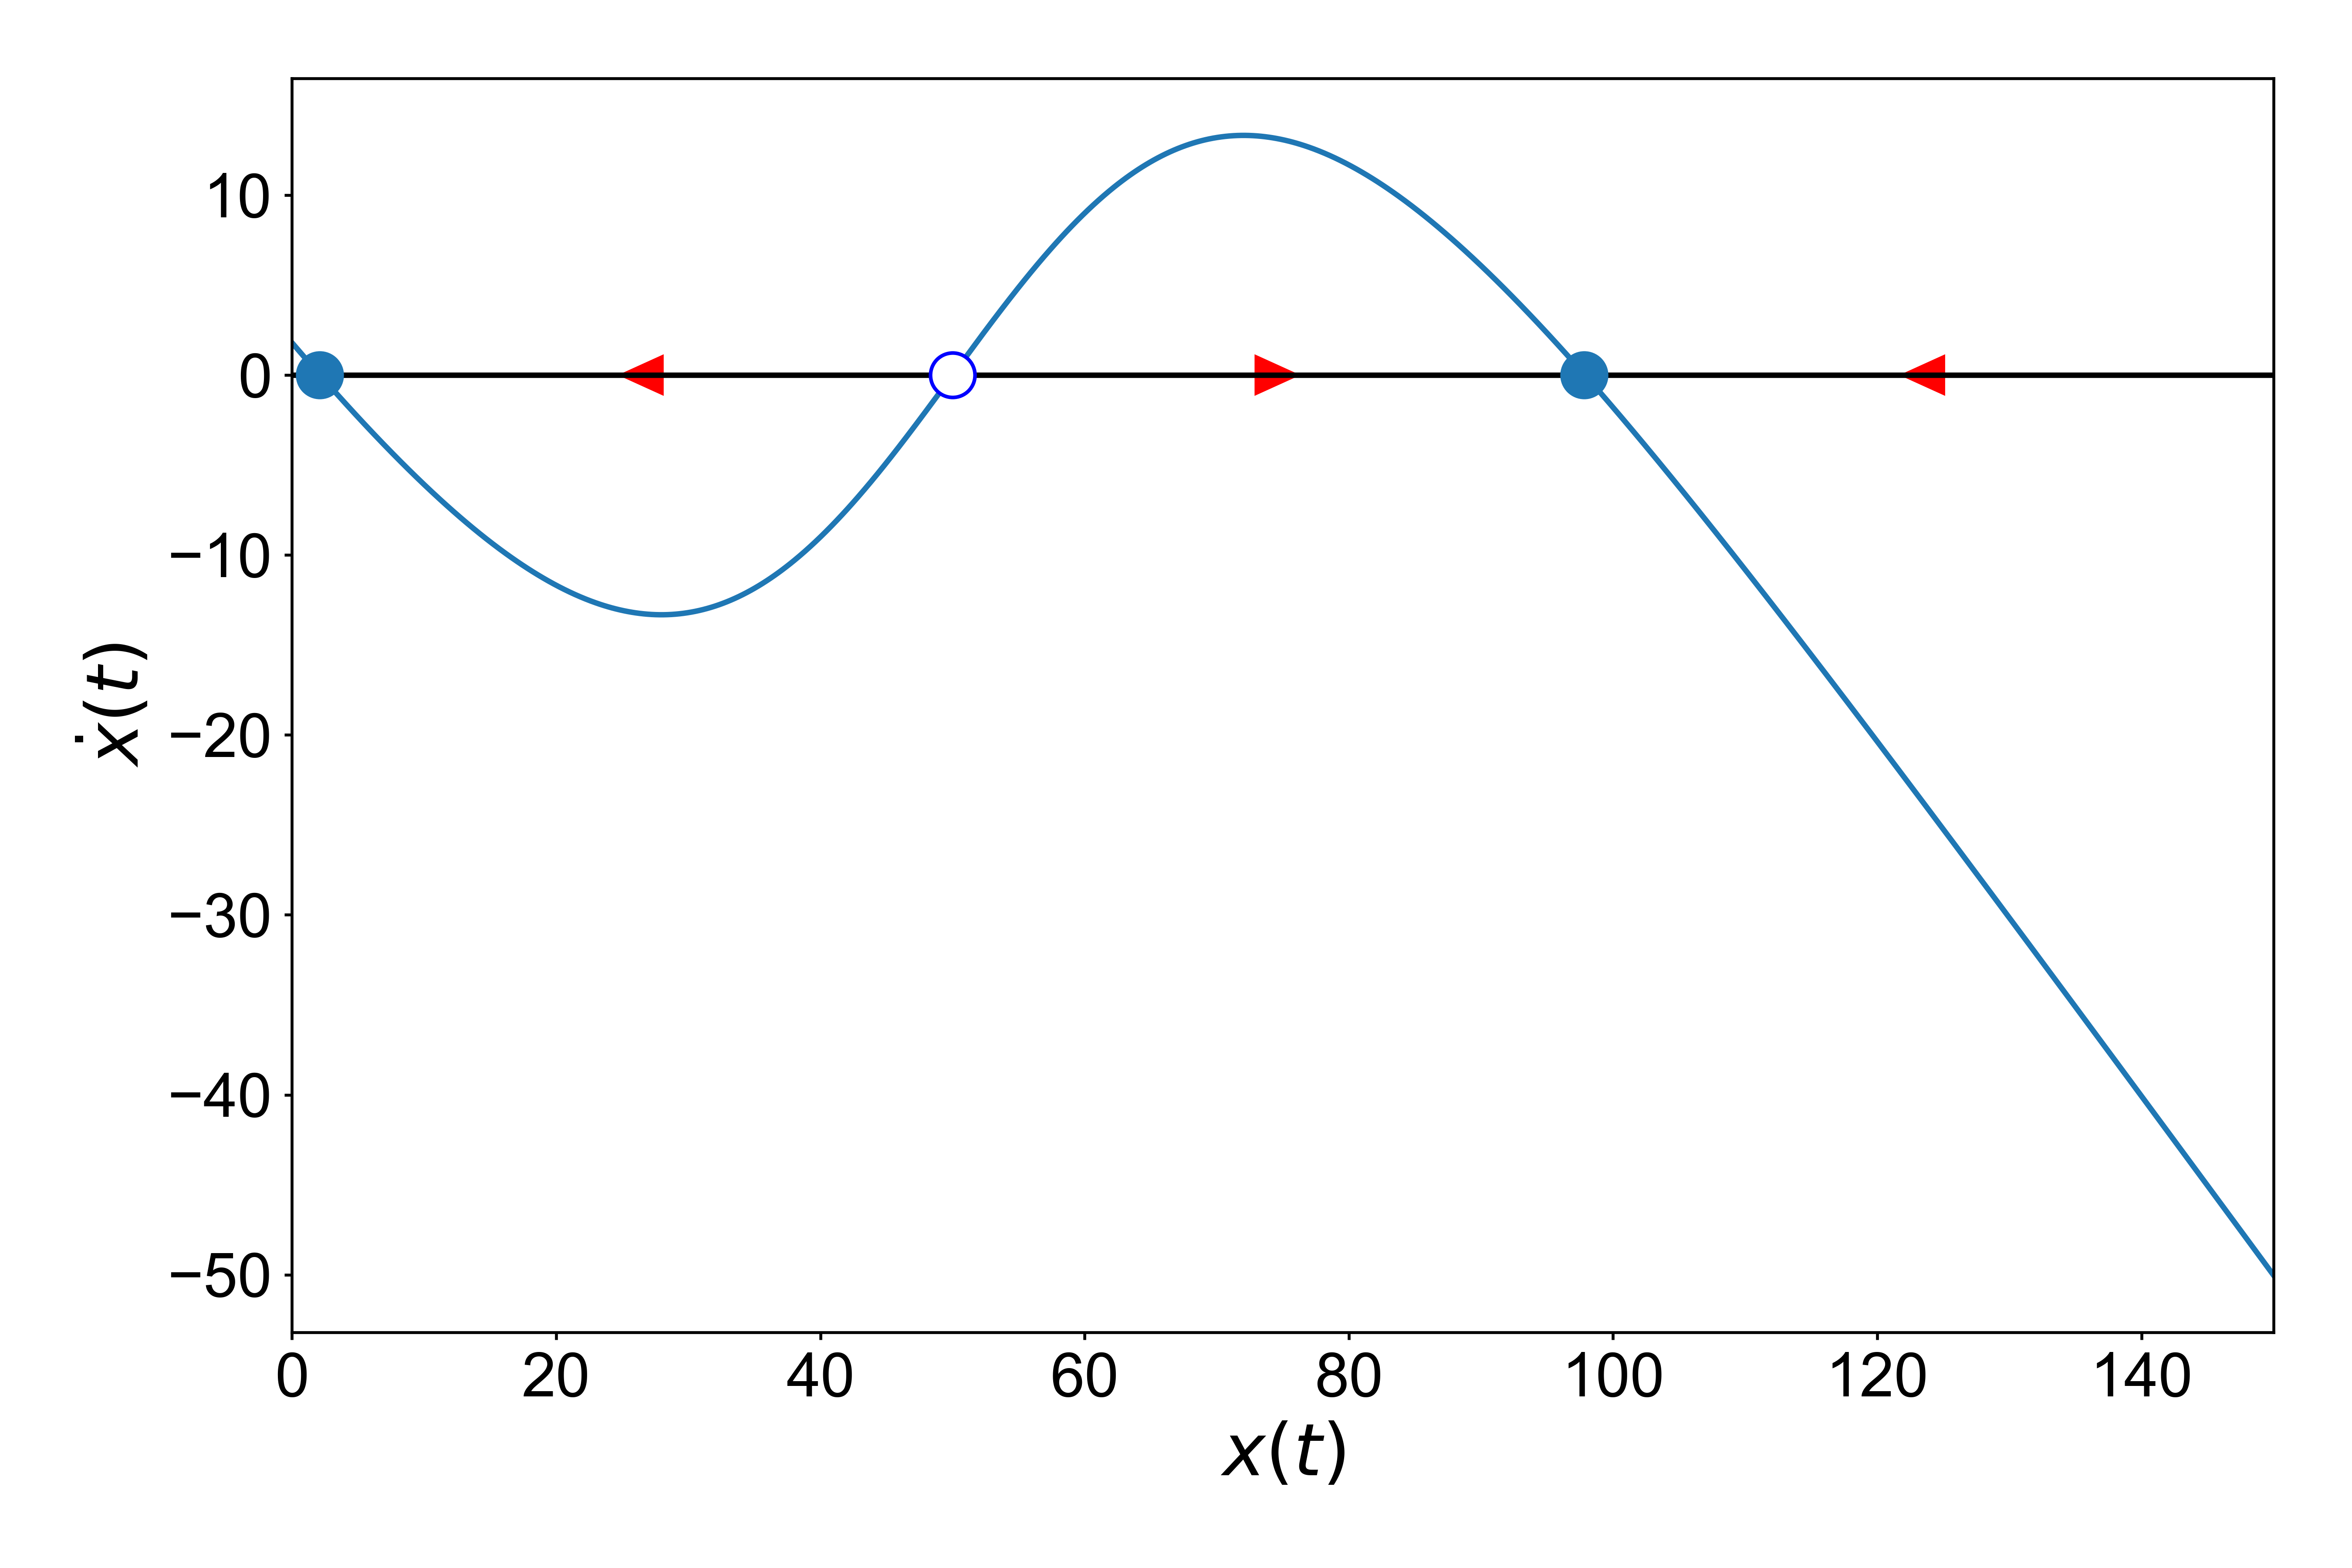
\includegraphics[width=.8\linewidth]{exercice5fig2.png}
\caption[spt]{Derivative $\dot{x}(t)$ as a function of $x(t)$: velocity field. Full dots show attractor and empty ones repellor fixed points.}\label{fig:fig2}
\end{figure}

Figure \ref{fig:fig2} also shows the fixed points of such a system are 2 attractors (2.12 and 97.88) and one repellor (50). Consequently if we simulate the system with either of those points as starting values, it is not going to evolve. However, if we simulate the system near the repellor point, e.g. 49 and 51, it is going to move away from this point to the next attractor point (Figure \ref{fig:fig3} Upper Left). If we want to be more realistic, we can add an error term to account for the stochasticity of neuronal activity. Let us add some standard gaussian noise $\eta(t)$ (of mean 0 and variance 1), modulated by a factor $\sigma$. Our system is then written as follows:

\begin{equation}\label{eq:3}
  \dot{x}(t) = -x(t) + f(wx(t) +I)+ \sigma\eta(t)
\end{equation}
\indent And the Euler approximation:
\begin{equation}\label{eq:4}
  {x}(t+1) = x(t) + (-x(t) + f(wx(t) +I))\delta t + \sigma \eta(t) \sqrt{\delta t}
\end{equation}

Consequently, for a small $\sigma$ (e.g. 0.5, Figure \ref{fig:fig3} Upper Right), a system starting from 49 or 51 will still tend towards 2.12 and 97.88 respectively. However, starting from 50, the stochasticity will bring the system away enough from the 50 repellor fixed point so that it will be attracted to the next attractor. Moreover, a higher $\sigma$ (e.g. 5, Figure \ref{fig:fig3} Lower Left), will make the system sometimes `cross` the 50 repellor, so that it will reach the attractors farther away from its starting point. And the stochasticity will make the system oscillates more broadly around the attractors too. For a great error factor $\sigma$ (e.g. 80, Figure \ref{fig:fig3} Lower Right), the system is overwhelmed by the error, so that only its oscillations are visible.

\begin{figure}[H]
\centering
\includegraphics[width=1\linewidth]{exercice5fig3.png}
\caption[spt]{Simulation of 10 seconds of the system for 30 trials with 3 possible starting point: $x_0$, 49,50, or 51. Dashed lines show the attractor fixed points. \textbf{From upper left to lower right:} $\sigma = 0$, $\sigma = 0.5$, $\sigma = 5$, $\sigma = 80$}\label{fig:fig3}
\end{figure}

We can try to interpret this considering our model represents a neuron's firing rate, with a constant inhibitory input current, and an autapse with a positive weight. This neuron will be able to sustain an elevated activity regime, i.e. to converge to a high firing rate ($\approx 98$ Hz), if its initial firing rate was greater than 50. However, it will have tend towards a sparse spiking activity state ($\approx 3$ Hz) if its initial firing rate was less than 50 Hz at the negtive input current onset. If its initial firing rate was exactly 50 Hz, it will stay stable, as it the input from itself compensate the negative input current ($0.04*50=2$).

%----------------------------------------------------------------------------------------
%	SECTION 2
%----------------------------------------------------------------------------------------

\section{Circuits with mutual inhibition}\label{circuits}
\indent\indent Let us now consider a little more complex system with two neurons, synapsing each other (but not themselves anymore). The following system of differential equation describes this, with $x_1$ the firing rate of the first neuron, and $x_2$ the firing rate of the second:

\begin{equation}\label{eq:5}
  \begin{cases}
    \dot{x_1}(t) = -x_1(t) + f(wx_2(t) +I)\\
    \dot{x_2}(t) = -x_2(t) + f(wx_1(t) +I)
  \end{cases}
\end{equation}

Using the dynamical system's approach again, we can look at the nullclines (values of the system so that $\dot{x_i}=0$), and the fixed points are the values for which $\dot{x_1} = \dot{x_2} =0$ (Figure \ref{fig:fig4}). We can use the same activation function as in section \ref{autapse}, use inhibitory weights $w=-0.1$ and a constant excitatory current $I=5$.

 When the system reaches those fixed points, both  neurons firing rate are remaining stable. Otherwise, if the system's is on one neuron's nullcline, it won't necessary `stay' there, as the second neuron's activity can make the system move away from it.

\begin{figure}[H]
\centering
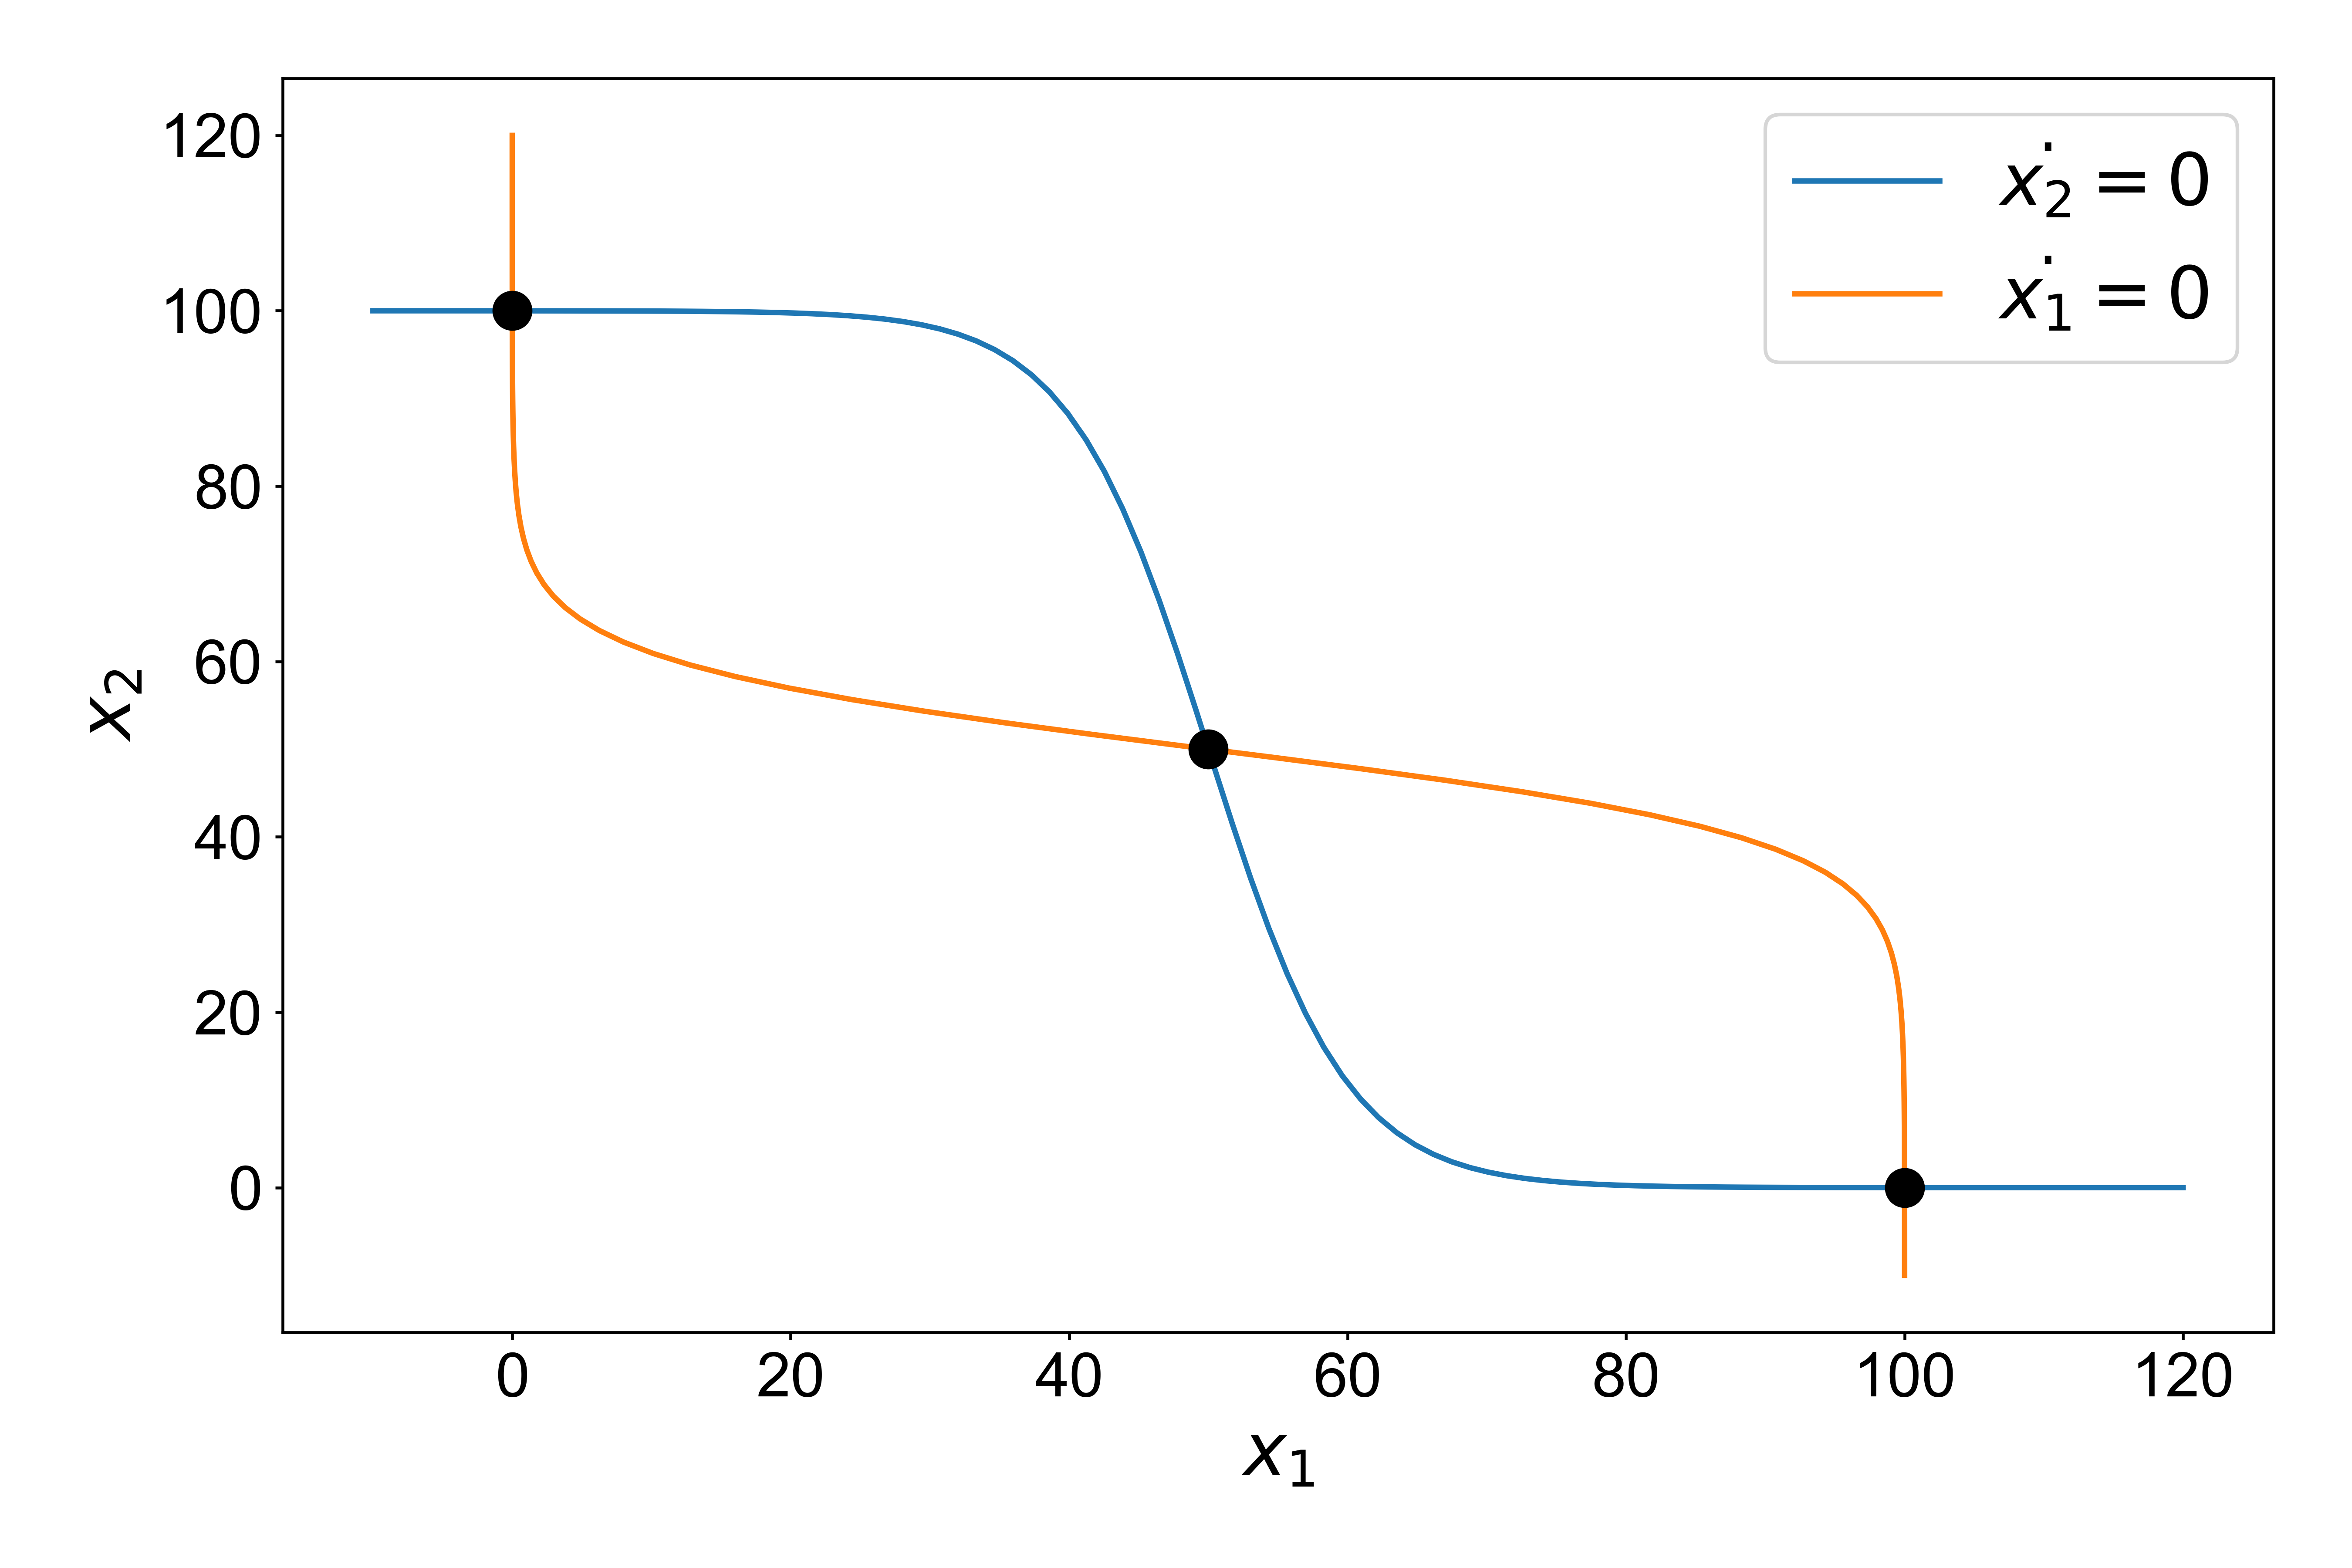
\includegraphics[width=.8\linewidth]{exercice5fig4.png}
\caption[spt]{Nullclines $\dot{x_1}=0$ and $\dot{x_2}=0$ as a function of $x_1$ and $x_2$. Full dots show fixed points.}\label{fig:fig4}
\end{figure}

To better capture the system's behavior, we can look at the trajectory of some starting points with different values of $x_1$ and $x_2$ (Figure \ref{fig:fig5}). It appears that the system is somewhat contained, that it tends towards a total firing rate of 100, with 3 possible combinations of firing rates $(x_1, x_2)$: (50,50), (100,0), (0,100). This makes sense as there is some sort of competition between the two neuron that inhibit each other. The one neuron that starts with the highest firing rate eventually overcome the other neuron's activity (Figure \ref{fig:fig6}). Interestingly, when the initial values of $x_1$ and $x_2$ are close to each other and under the 50-50 repellor point(Figure \ref{fig:fig5}), it seems they grow at the same rate, until they near the mentioned repellor, after that their trajectories differ. This effect is probably due to the sigmoidal form of the activation function. \\

\begin{figure}[H]
\centering
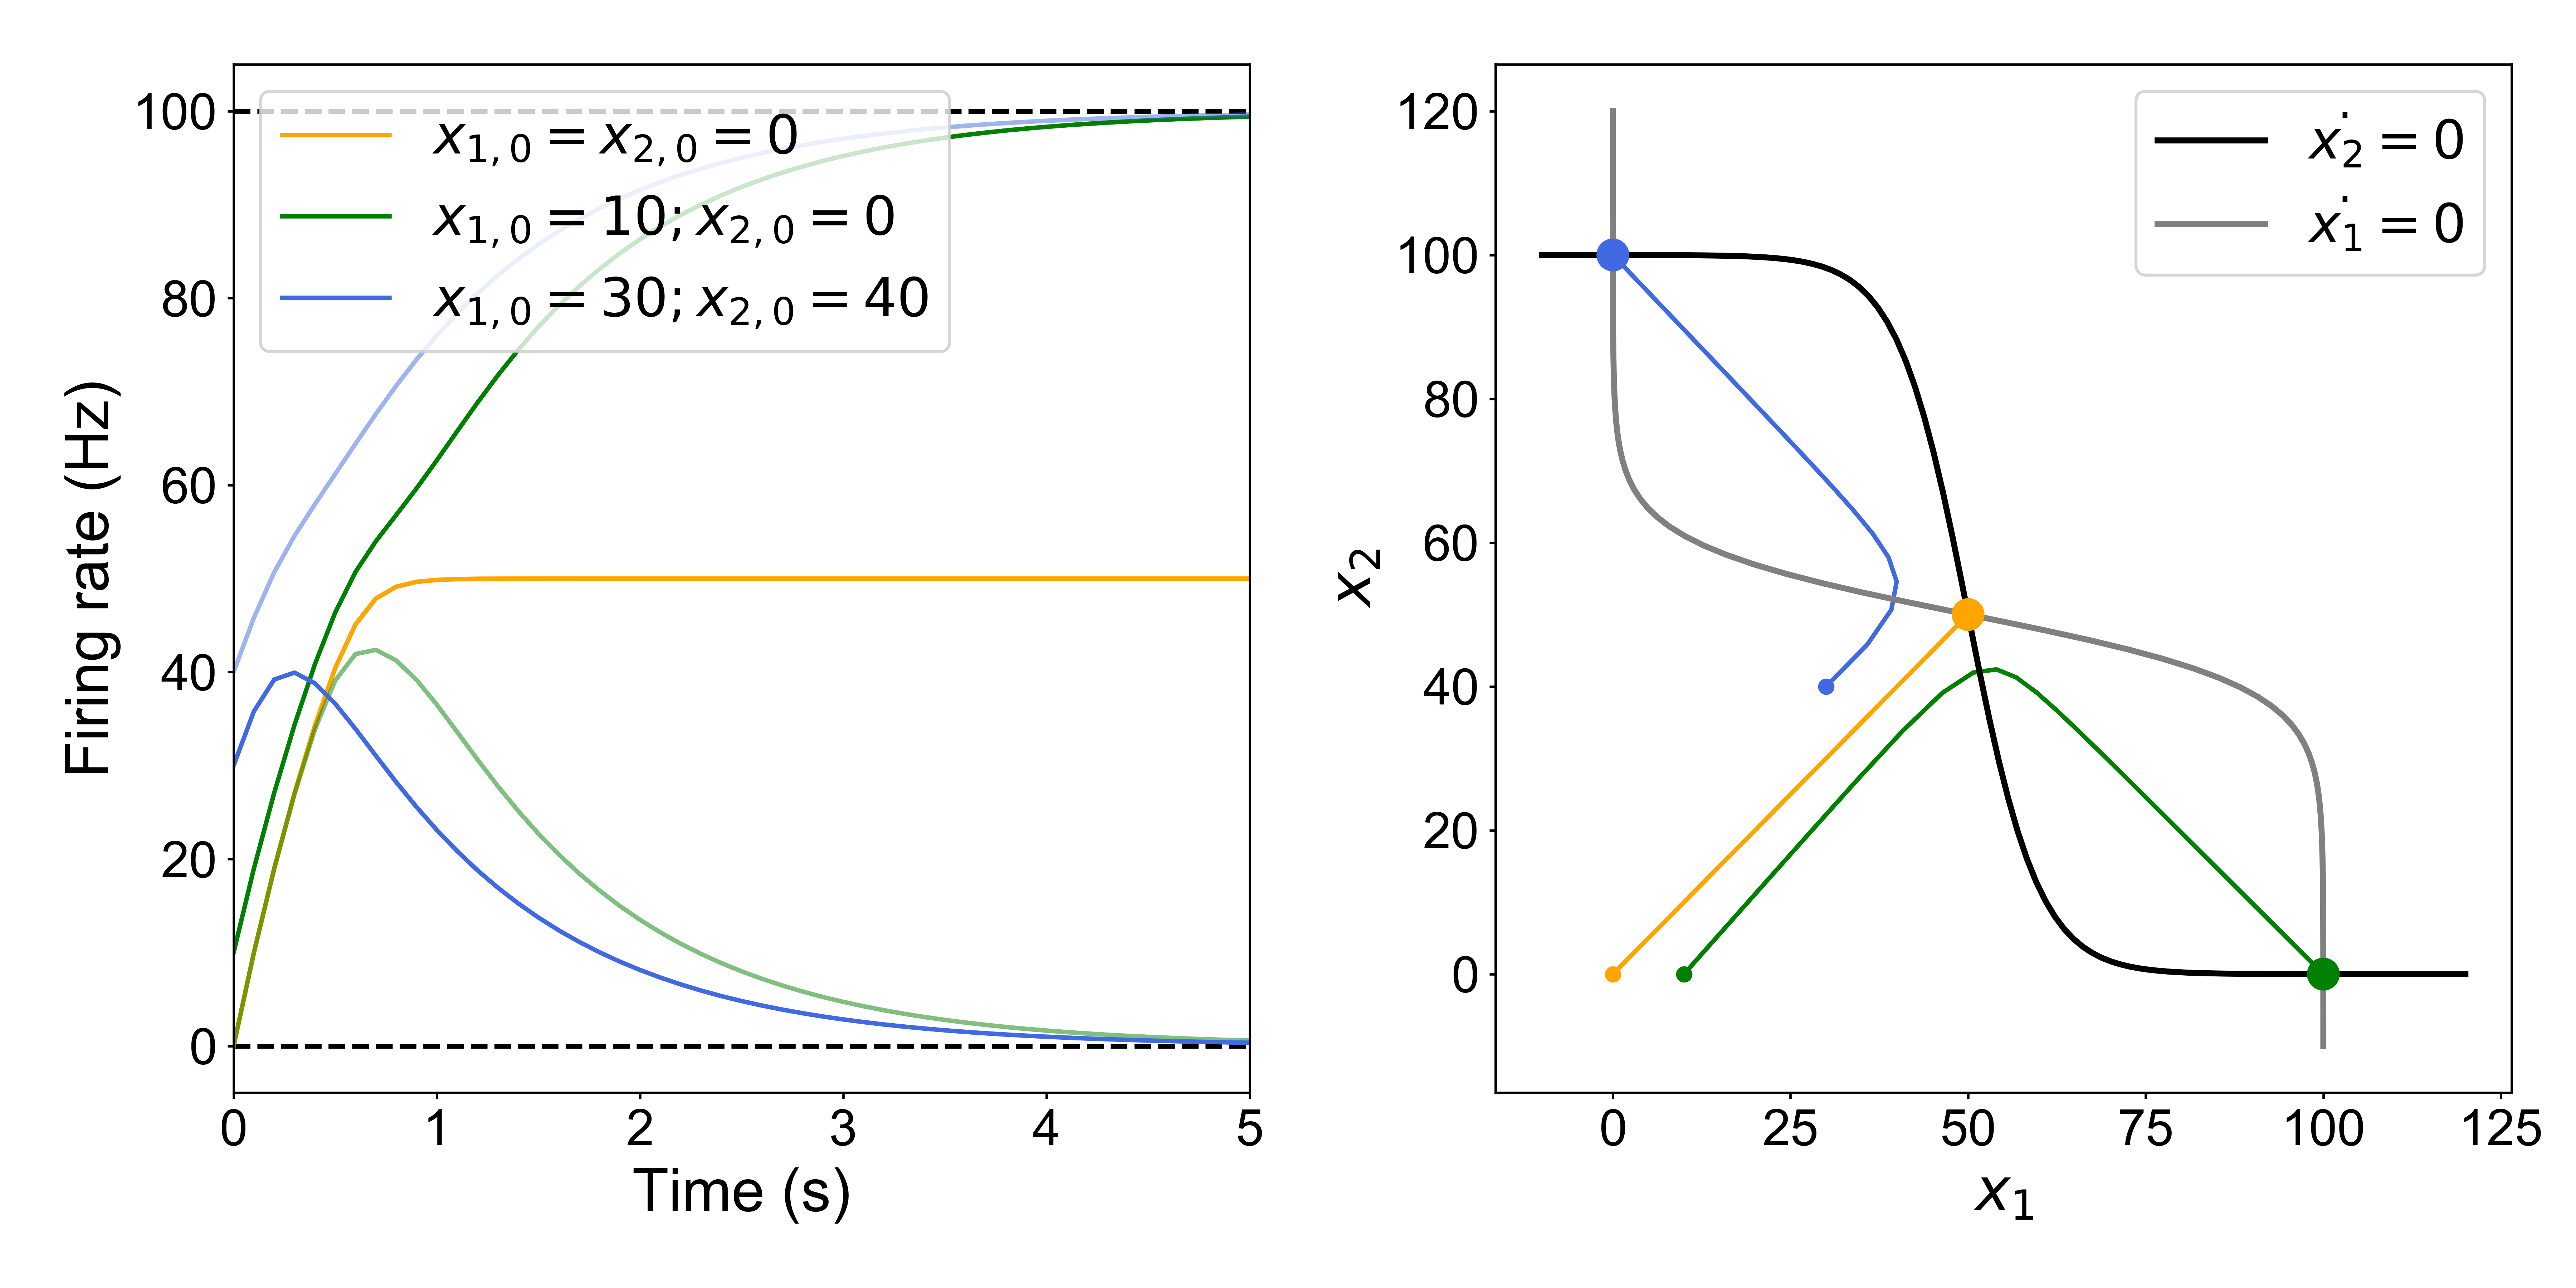
\includegraphics[width=1\linewidth]{exercice5fig5.png}
\caption[spt]{\textbf{Left} Firing rate in time, of neuron 1 (dark colored) and 2 (light colored), for different starting values. \textbf{Right} Trajectory of the two firing rates in $(x_1, x_2)$ space}\label{fig:fig5}
\end{figure}

Moreover, if the initial firing rates are equal, the combined firing rates point in $(x_1, x_2)$ space, stays on the line $x_1 = x_2$ and reach progressivelly the 50-50 repellor point, as no neuron manage to overcome the other (Figure \ref{fig:fig6}, note that there is no noise in this model).

\begin{figure}[H]
\centering
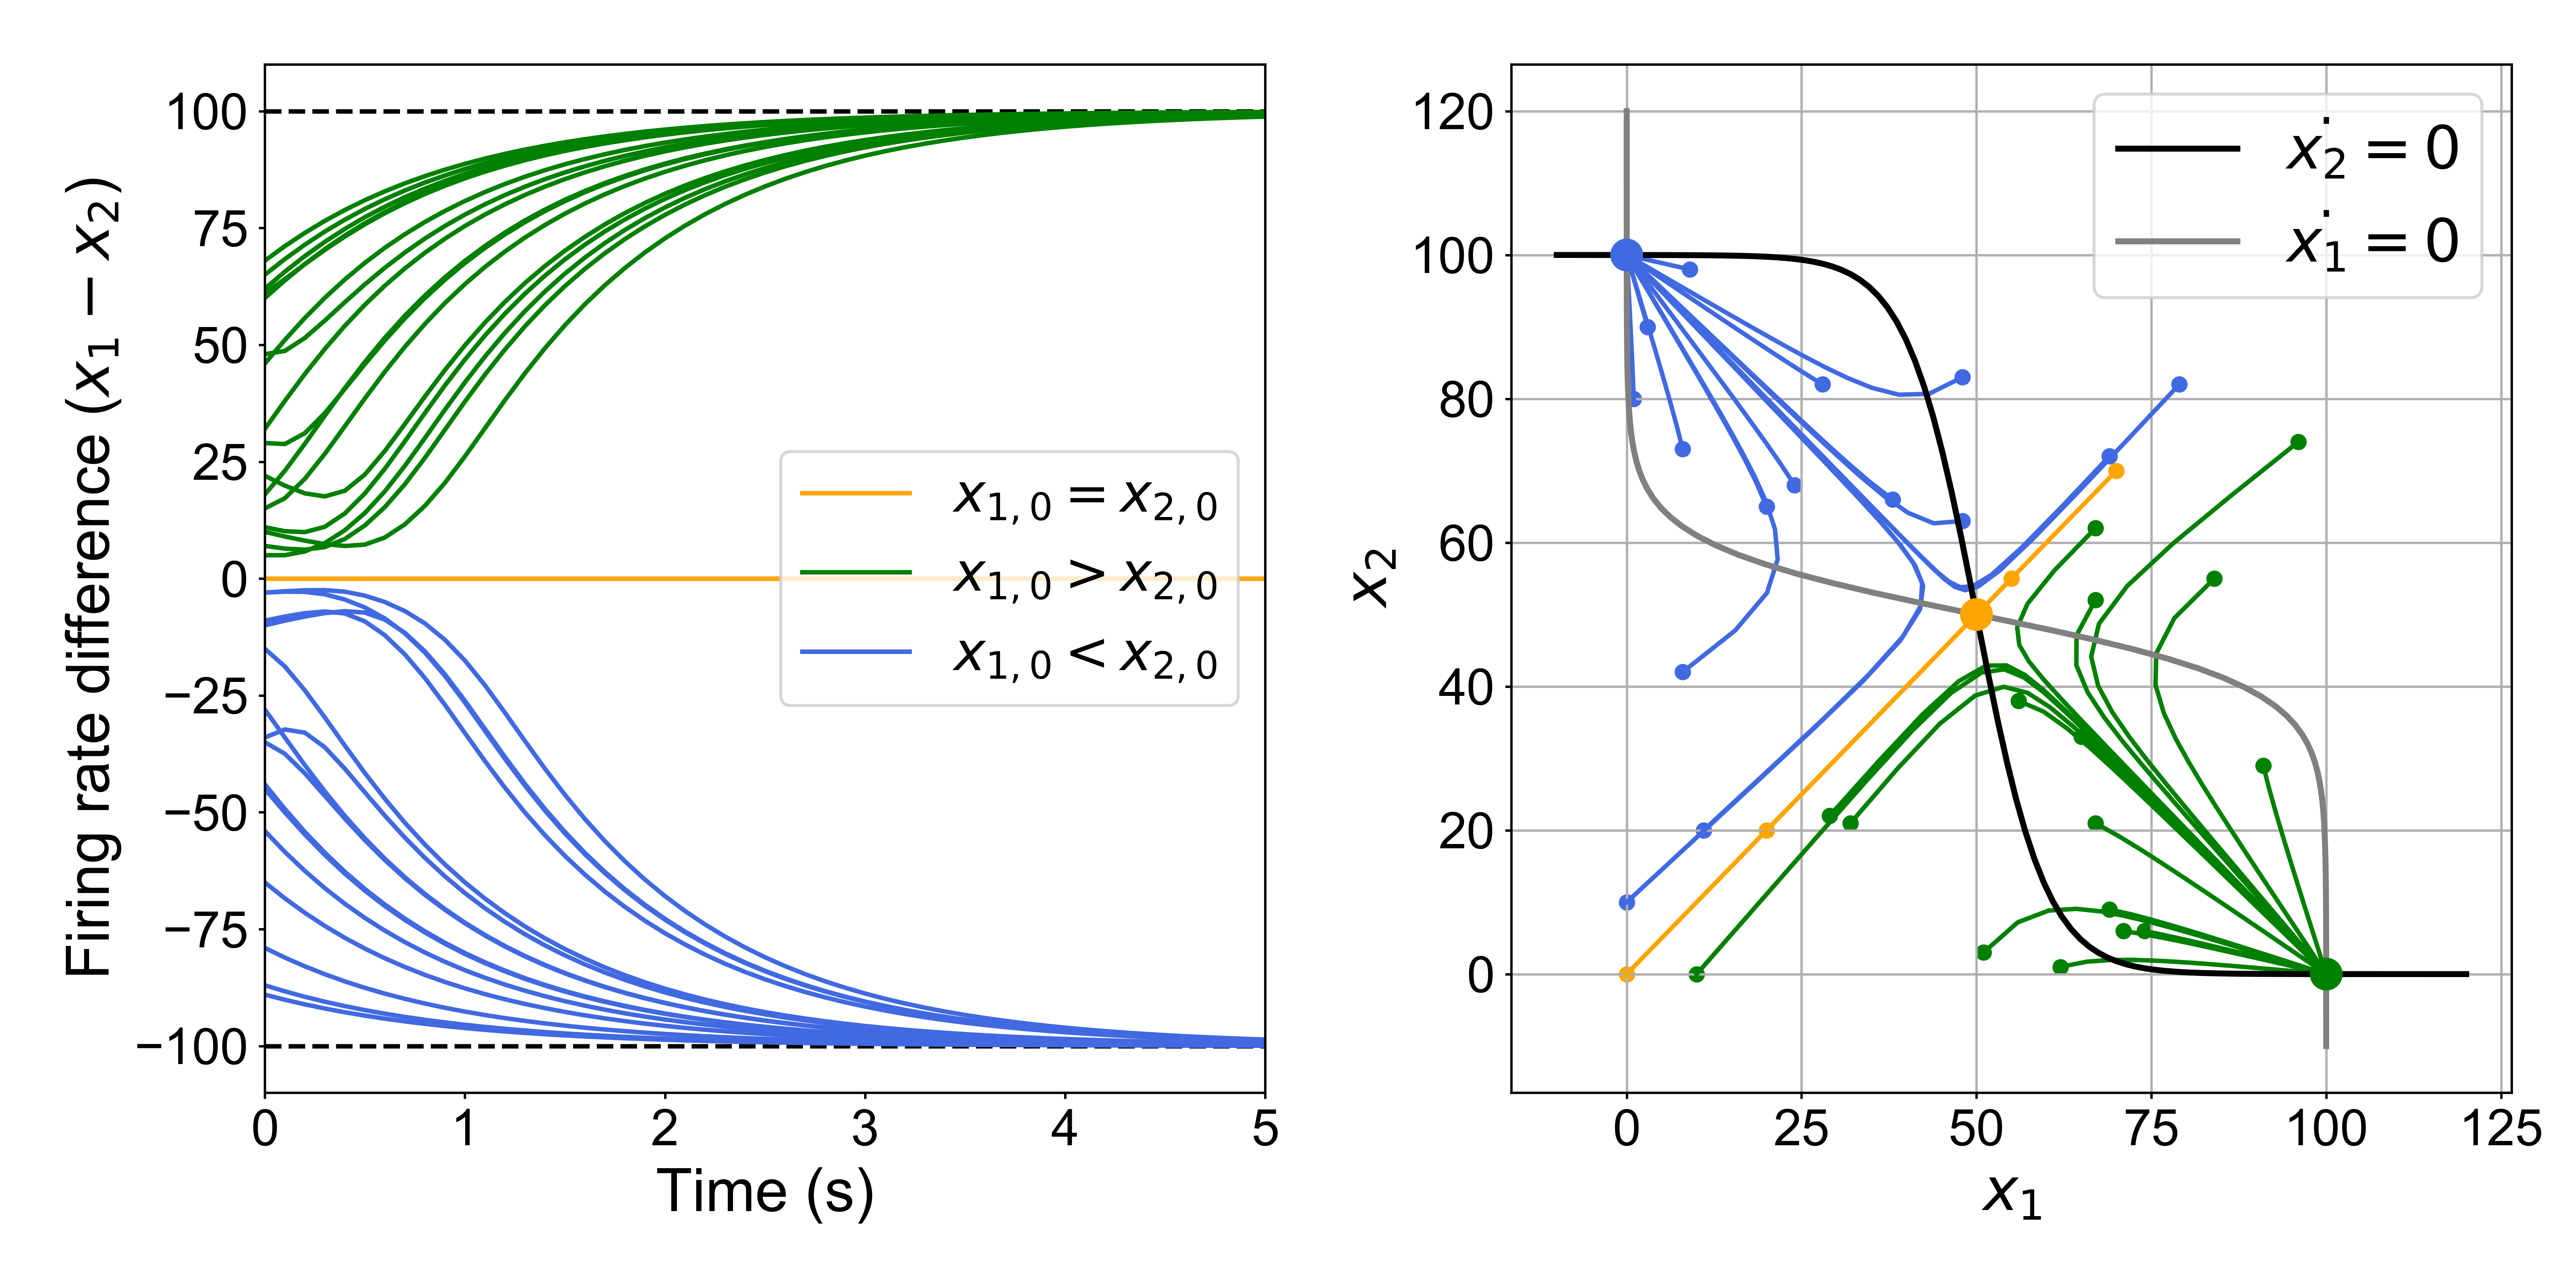
\includegraphics[width=1\linewidth]{exercice5fig6.png}
\caption[spt]{\textbf{Left} Difference of firing rate  of neuron 1 and 2 in time, for different starting values. \textbf{Right} trajectory of the corresponding firing rates in $(x_1, x_2)$ space}\label{fig:fig6}
\end{figure}

Another way to visualize the networks dynamics is to look at the velocity field, similarly to Figure \ref{fig:fig2} but with more dimensions (Figure \ref{fig:fig7}). The flow(s) seems to confirm our previous observations.

\begin{figure}[H]
\centering
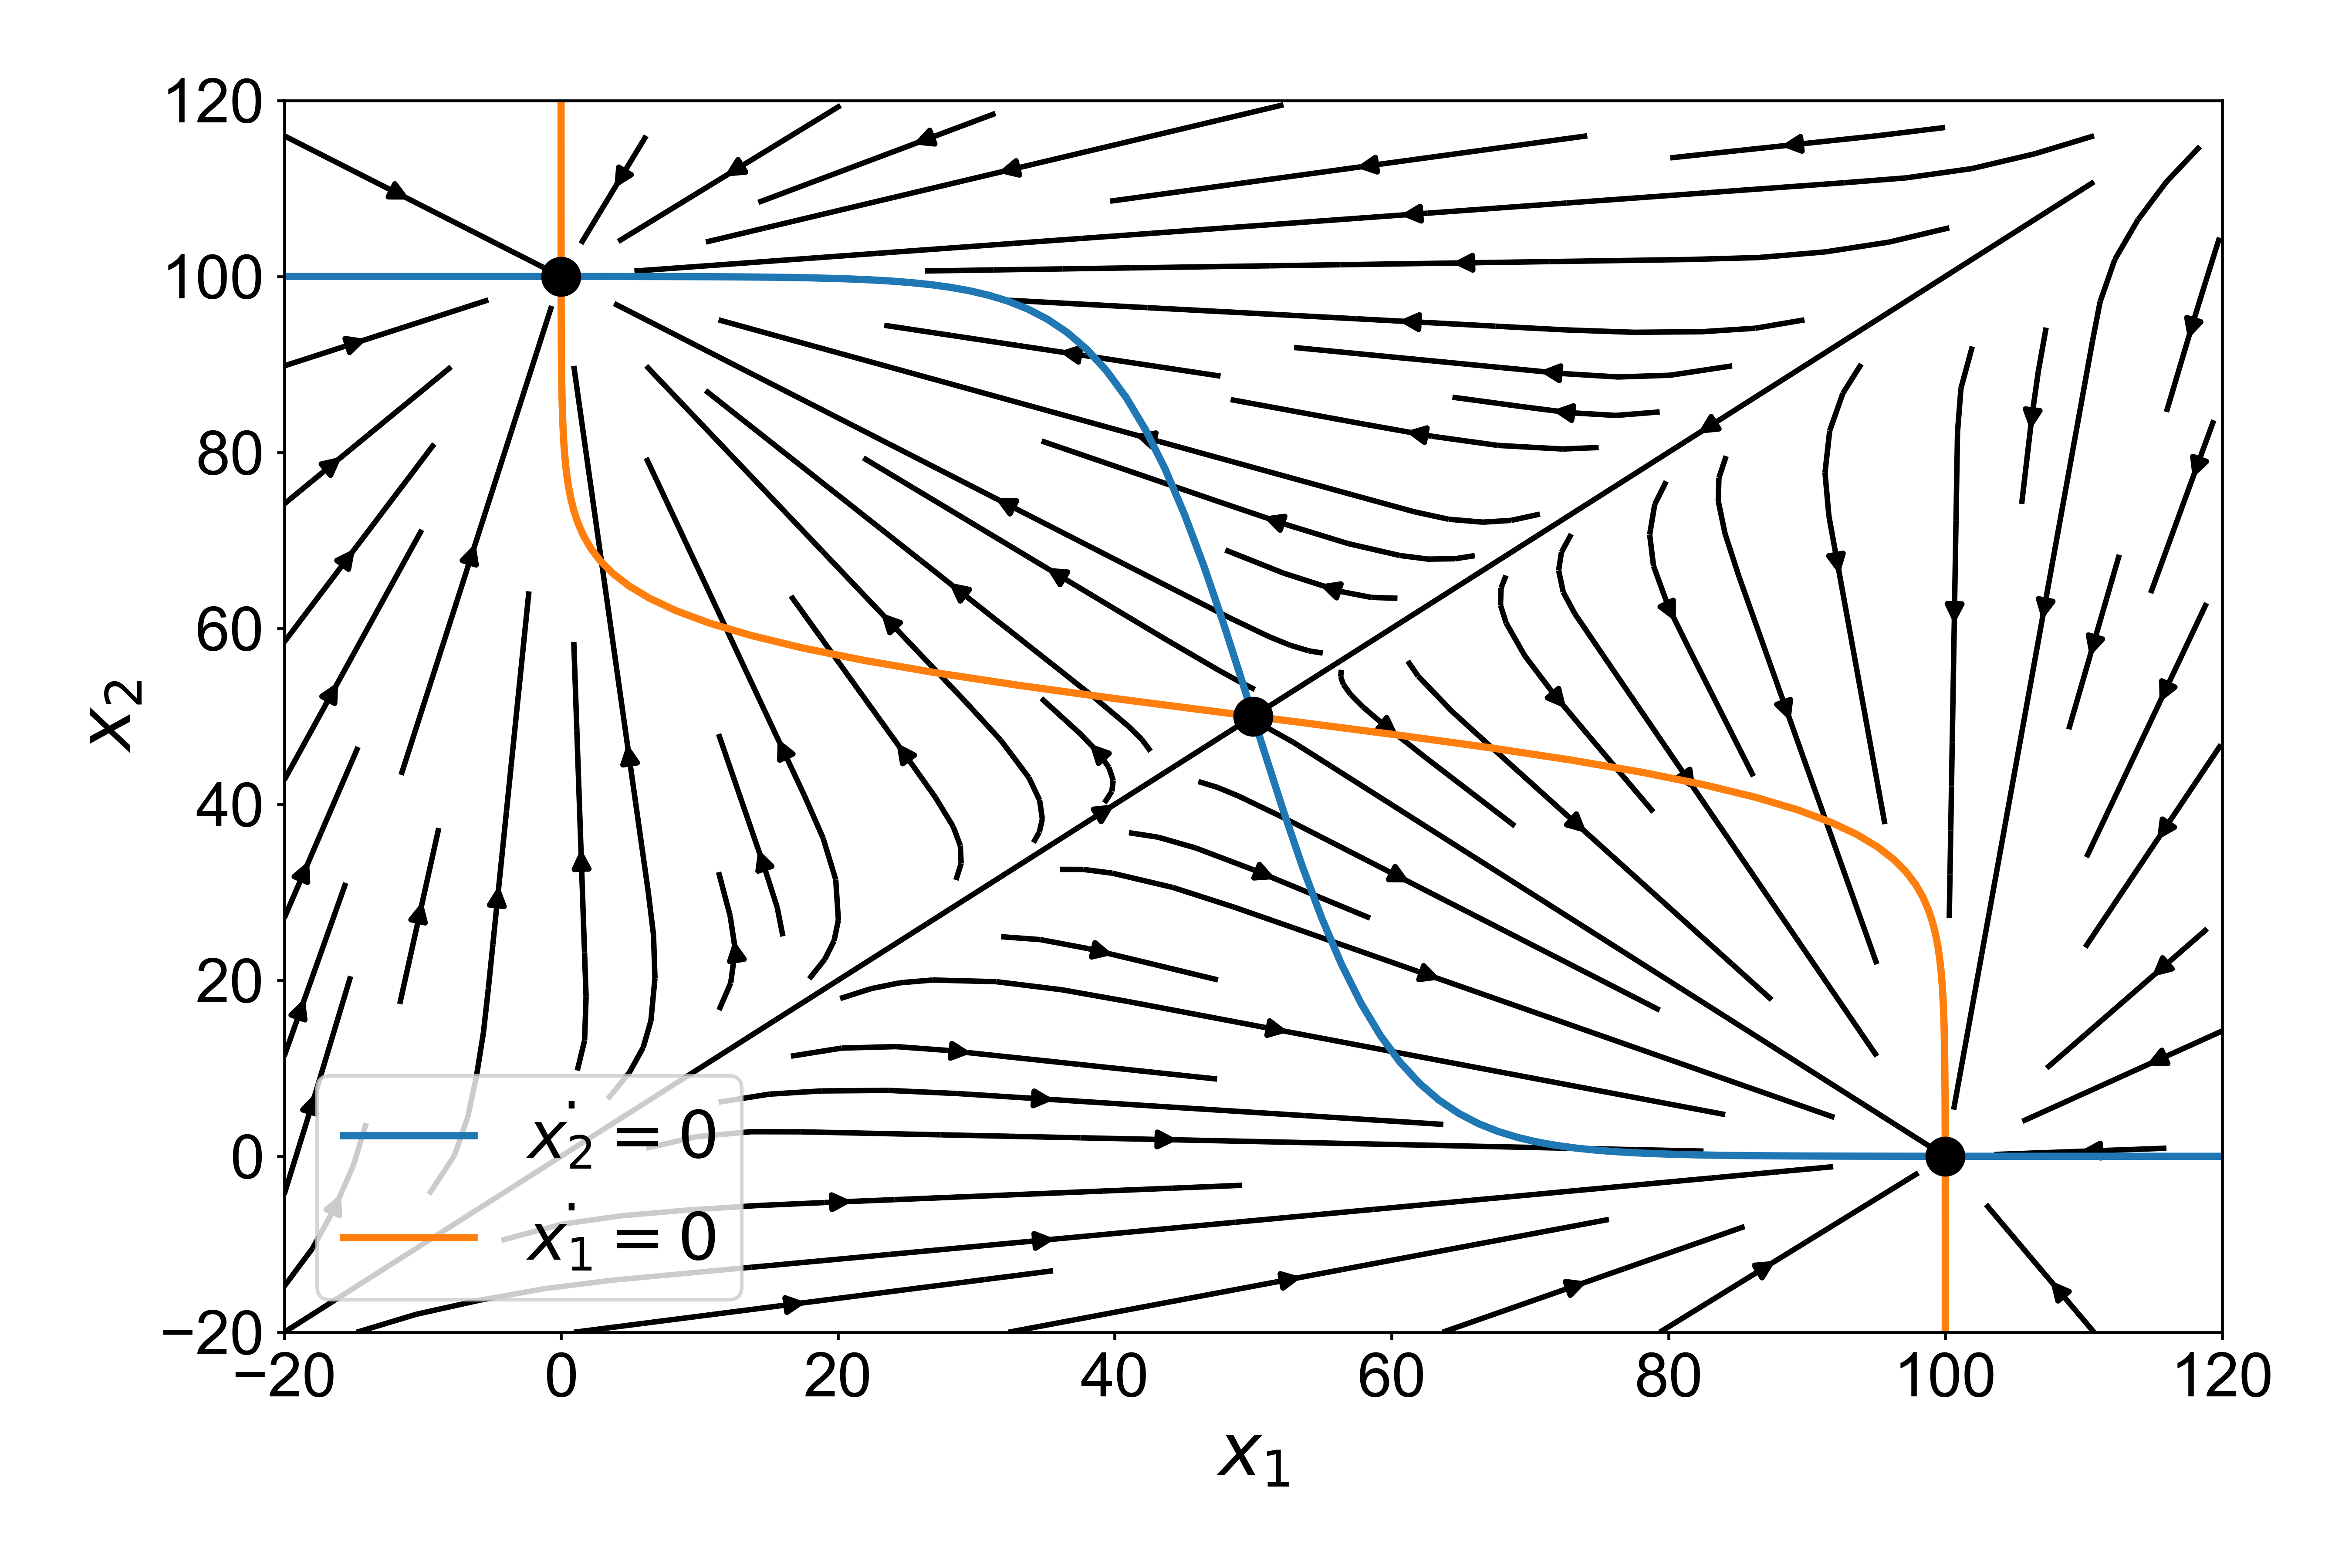
\includegraphics[width=1\linewidth]{exercice5fig8.png}
\caption[spt]{Velocity field of the dynamic system $(x_1, x_2)$.}\label{fig:fig7}
\end{figure}

Now, regarding the code to model the dynamics of the network, there are several options available. Let's take Figure 5 parameters:

\begin{lstlisting}[language=Python, caption=Parameters]
w=-.1; I= 5; dt=.1
x0_1=[0,10,30]; x0_2=[0,0,40]
\end{lstlisting}
\indent Now for the 3 initial values, we can have 50 iterations (5 seconds) of a loop updating the system with the Euler method, and stocking the values at each point in two array:
\begin{lstlisting}[language=Python, caption=System dynamics]
xt1=x0_1[i]
xt2=x0_2[i]
x_array1 = [xt1]
x_array2 = [xt2]
for j in range(50):
    xt1 += (-xt1 + f(w*xt2+I)) *dt
    xt2 += (-xt2 + f(w*xt1+I)) *dt
    x_array1.append(xt1)
    x_array2.append(xt2)
\end{lstlisting}

Then you can easily plot the firing rate and the trajectory in $(x_1, x_2)$ space for each initial values:
\begin{lstlisting}[language=Python, caption=Plots]
#firing rate in time
plt.plot(np.linspace(0,5, 51),x_array1)
#trajectory
plt.plot(x_array1, x_array2)
\end{lstlisting}

However, a more comprehensive approach is to use matrices and arrays (of arrays):
\begin{equation}\label{eq:6}
    \dot{\mathbf{x}}(t) = -\mathbf{x}(t) + f(W \mathbf{x}(t) + I)
\end{equation}
Now in python code:
\begin {lstlisting}[language=Python, caption=Parameters]
W=np.mat('0 -0.1; -0.1 0')
x0=np.array([[0,0], [10,0], [30,40]])
\end{lstlisting}

\begin{lstlisting}[language=Python, caption=System]
xt=x0[j]
x_array = np.array(np.array(xt))
plt.figure(1)
for i in range(50):
    dxt= np.squeeze(f(np.array(np.dot(W,xt))+I))
    xt = xt + np.dot((-xt + dxt),dt)
    x_array = np.vstack([x_array, xt])
\end{lstlisting}

\begin{lstlisting}[language=Python, caption=Plots]
#firing rate in time
plt.plot(np.linspace(0,5, 51),x_array[:,0])
#trajectory
plt.plot(x_array[:,0], x_array[:,1])
\end{lstlisting}

%----------------------------------------------------------------------------------------
%	SECTION 3
%----------------------------------------------------------------------------------------

\section{Hopfield model}\label{hopfield}
\indent\indent Let's now consider a network of 64 neurons, each connected to themselves and to each other (so with 64² weights). If consider the activity of the a neuron at time t depends on the inputs from all the neurons at time t-1, the network is then called synchronous. Moreover, we can simplify neuronal activity by using $f(x)=sign(x)$ as an activation function to scale the activity between -1 and 1. Such networks are called Hopfield networks from its creator, but there are many types of such networks possible.\\
\indent In our case, we can give the dynamics of the network by the following differential equation:
\begin{equation}\label{eq:7}
    \dot{\mathbf{x}}(t) = -\mathbf{x}(t) + f(W \mathbf{x}(t)) + \sigma \eta(t)
\end{equation}
\indent And the Euler approximation:
\begin{equation}\label{eq:8}
  \mathbf{x}(t+1) = \mathbf{x}(t) + (-\mathbf{x}(t) + f(W\mathbf{x}(t)))\delta t + \sigma \eta(t) \sqrt{\delta t}
\end{equation}

Such a network can store `patterns' of activity in its weights, such that, for any starting pattern, the network converges to the pattern stored. Hopfield also designed a method to set the weights so that a given pattern $\mathbf{p}$ is stored in it:

\begin{equation}\label{eq:9}
  W=\frac{1}{N}\mathbf{p}\mathbf{p}^T
\end{equation}
where N is the number of cells.\\

Let's define 2 patterns $p$ and $q$ (thumbs up and down; beige =-1, blue=1):

\begin{figure}[H]
\centering
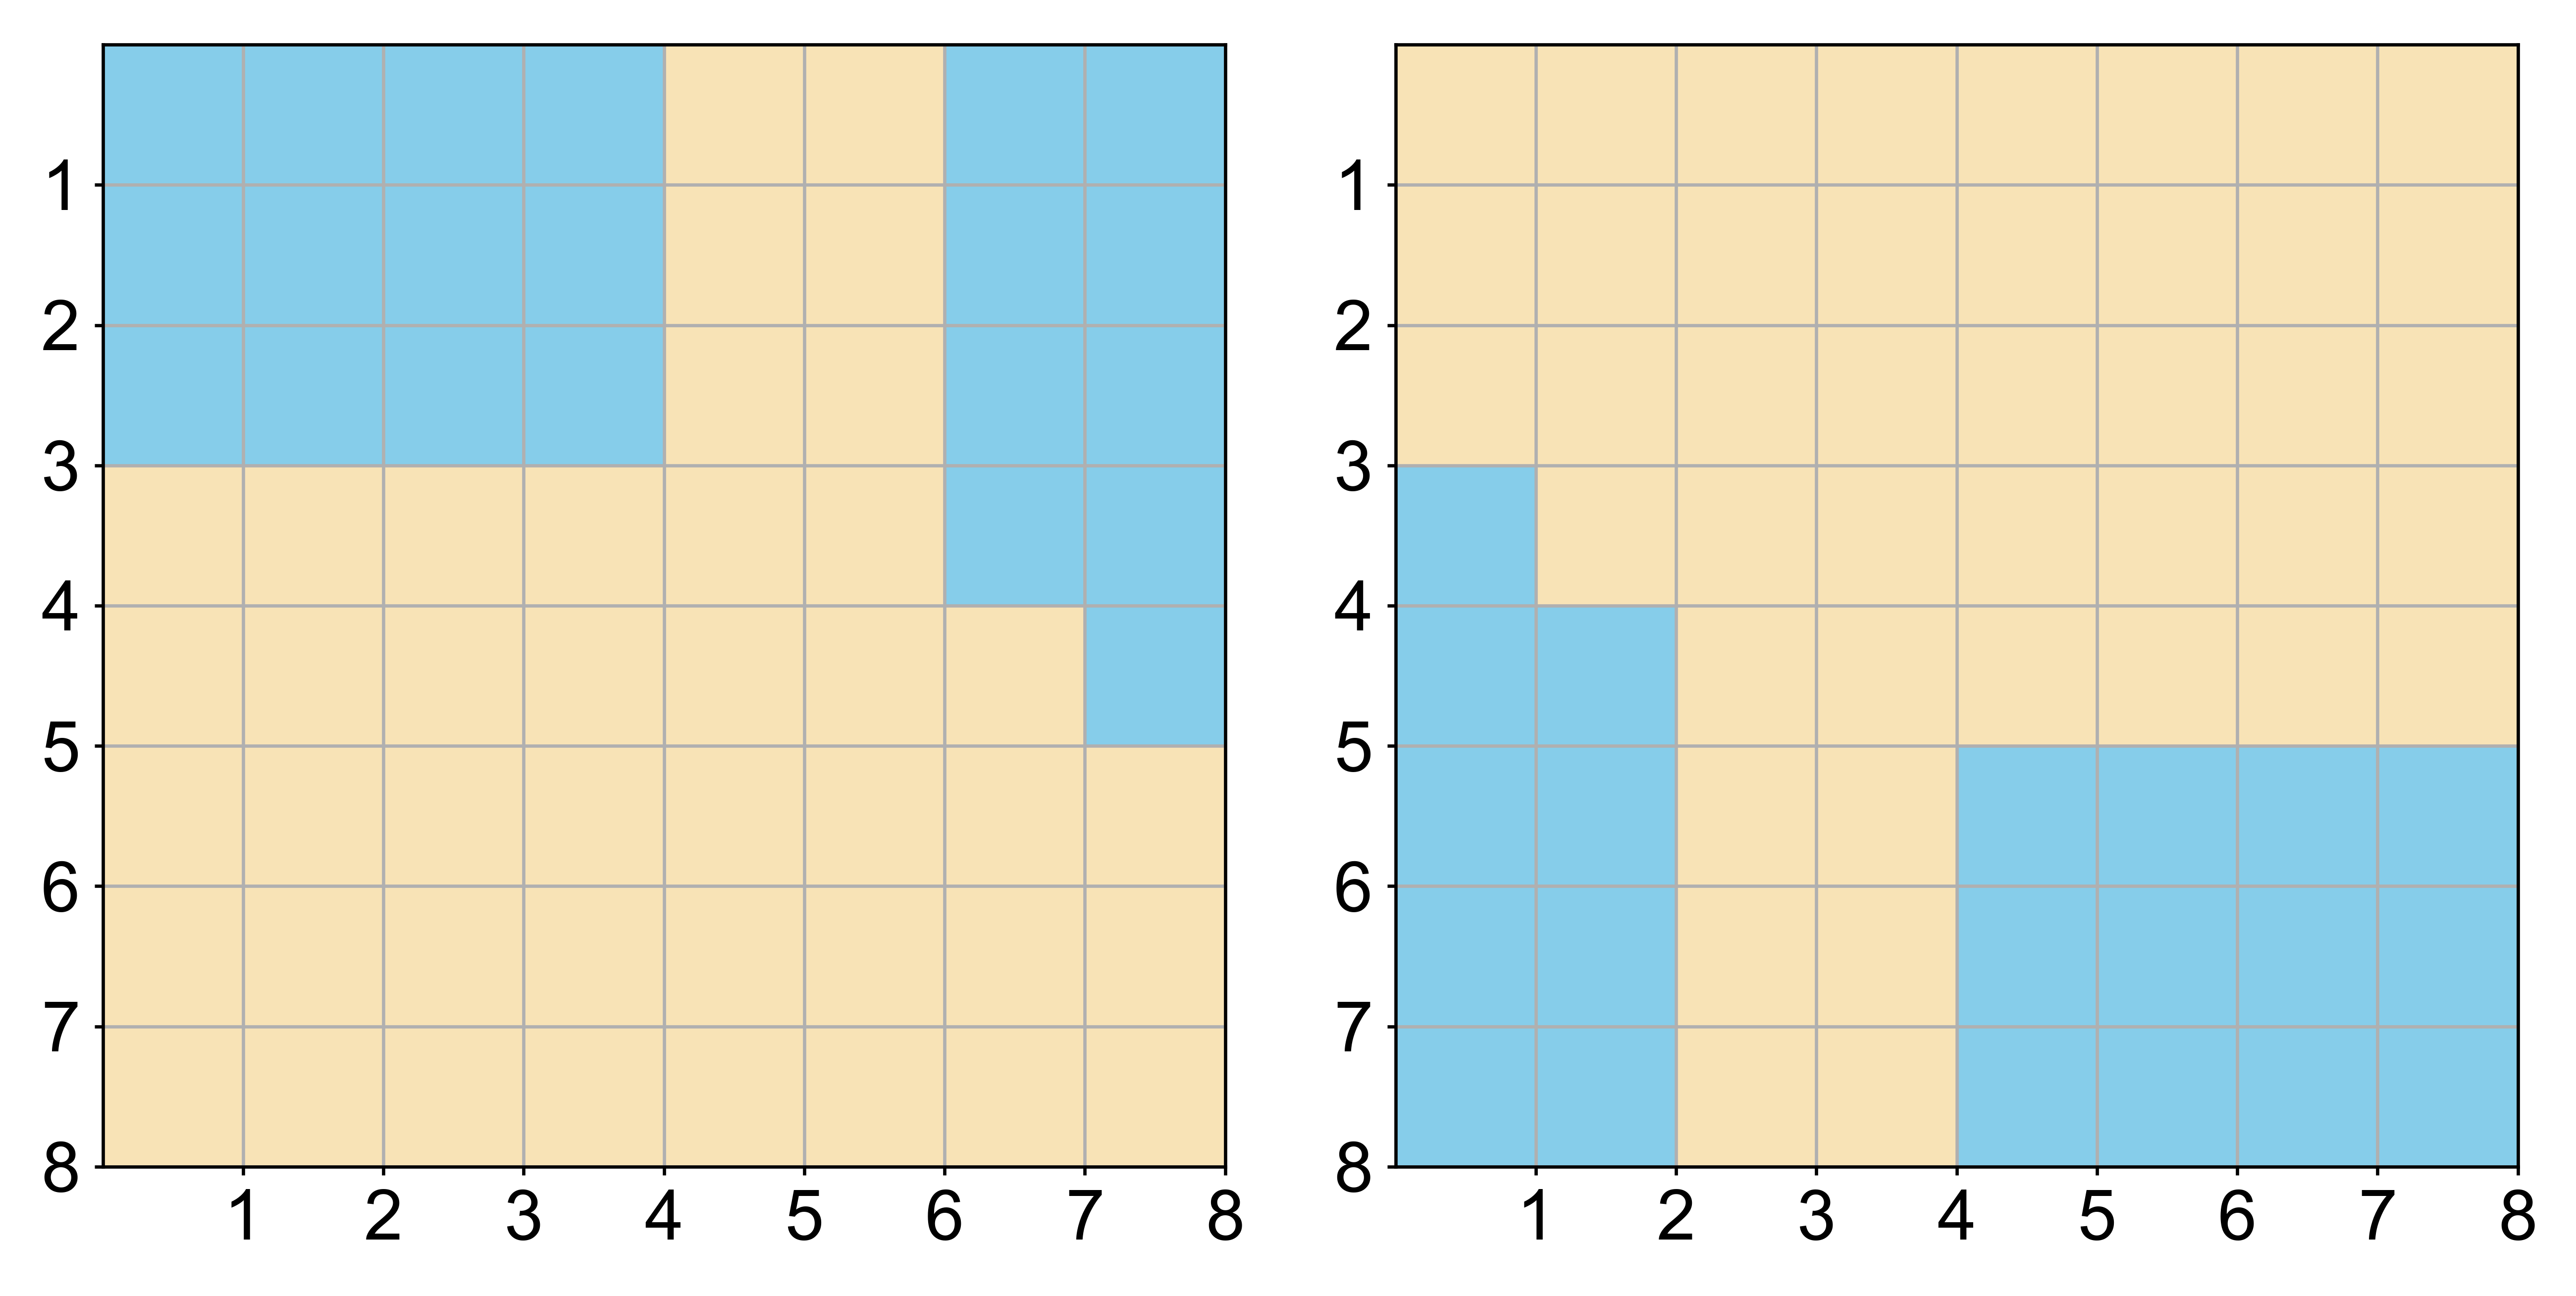
\includegraphics[width=.8\linewidth]{exercice5fig9.png}
\caption[spt]{Patterns $p$ (left) and $q$ (right)}\label{fig:fig8}
\end{figure}

If we set the weights according to equation (\ref{eq:9}), $\delta t = .1$, and $\sigma=.1$; and simulate the networks from a random pattern, it stabilizes to 2 patterns: $p$ and $-p$ (Figure \ref{fig:fig9} and \ref{fig:fig10}). It depends on the initial initial pattern closeness to either.

\begin{figure}[H]
\centering
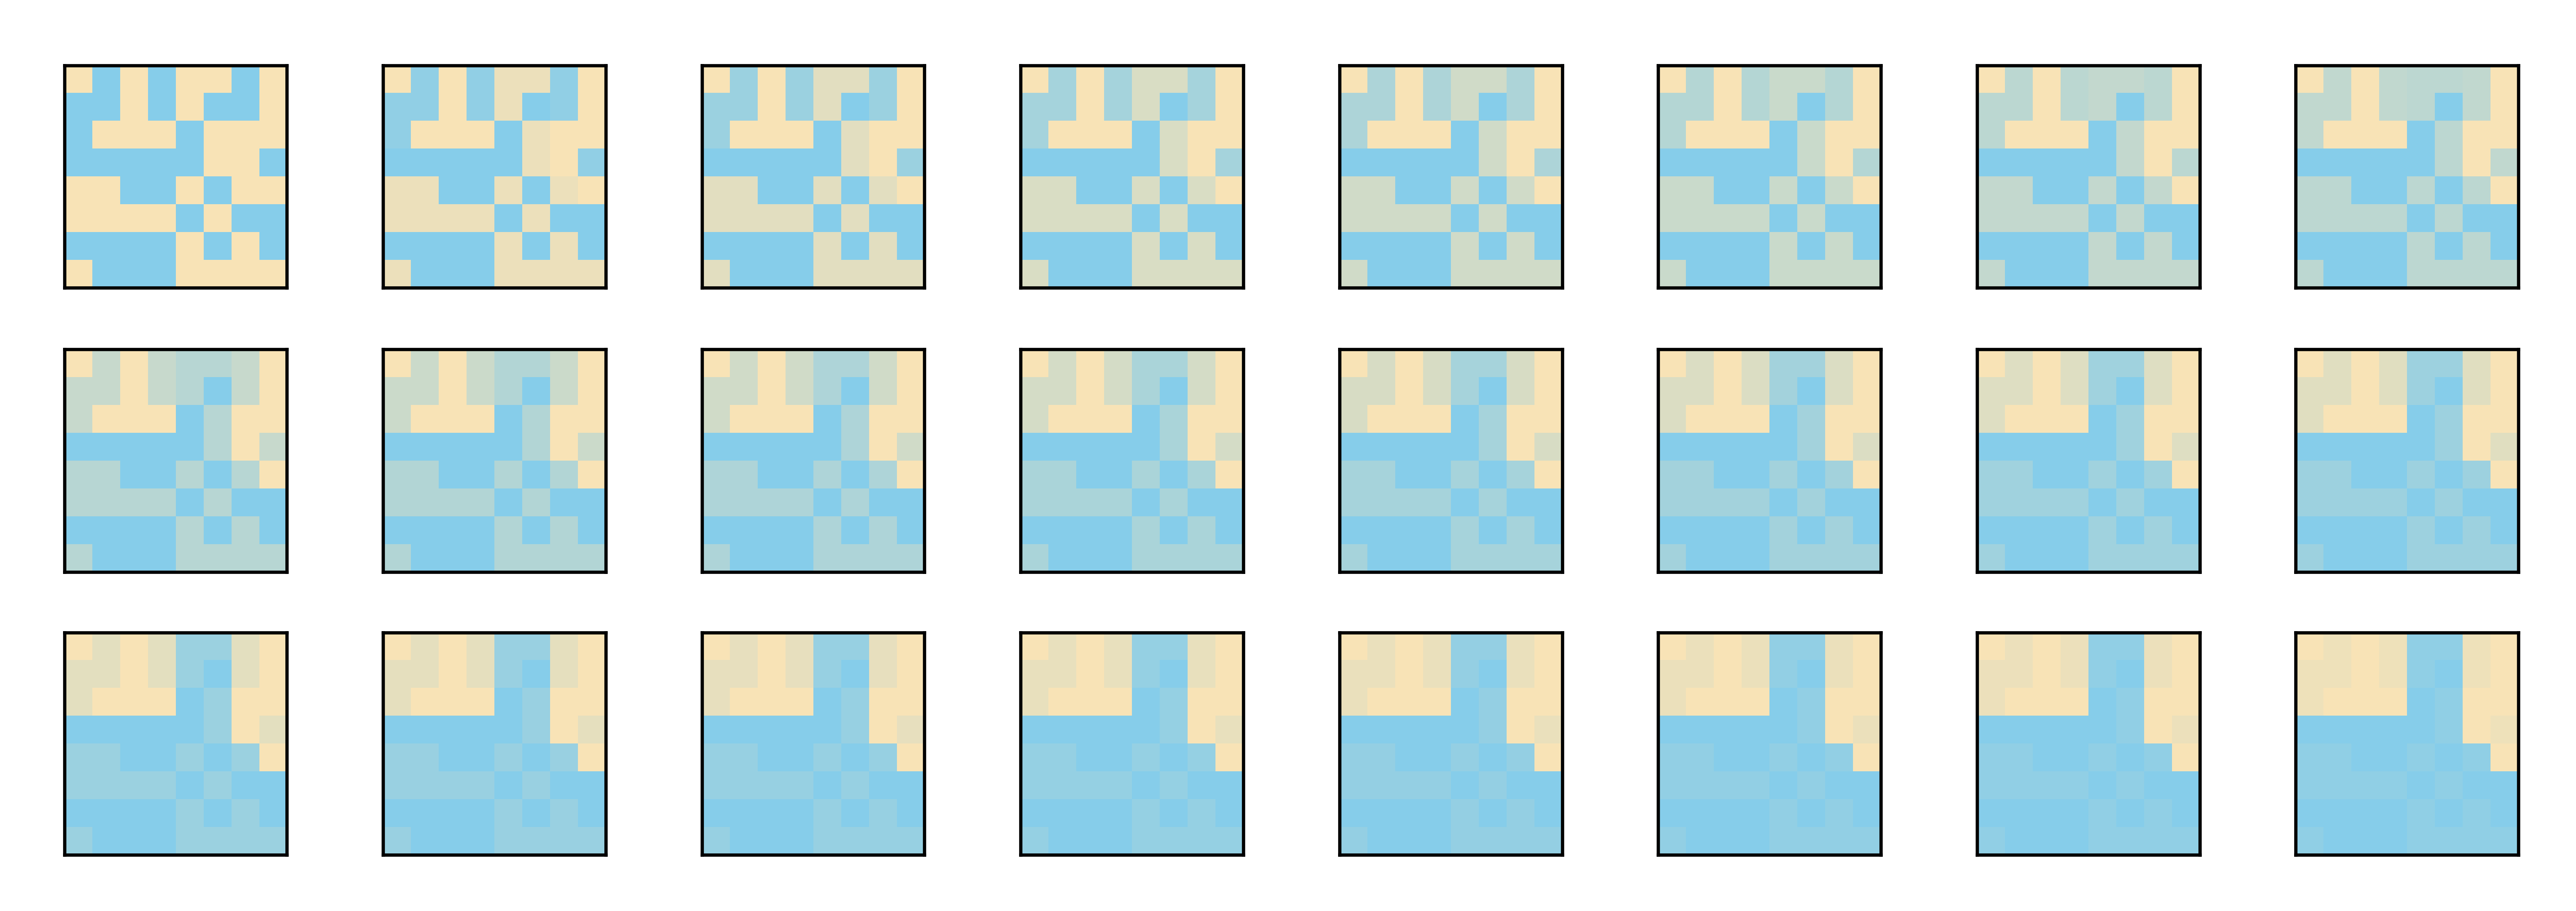
\includegraphics[width=.8\linewidth]{exercice5fig10.png}
\caption[spt]{From upper left to lower right, the network described above for 23 iterations of its dynamics, from a random initial pattern}\label{fig:fig9}
\end{figure}

\begin{figure}[H]
\centering
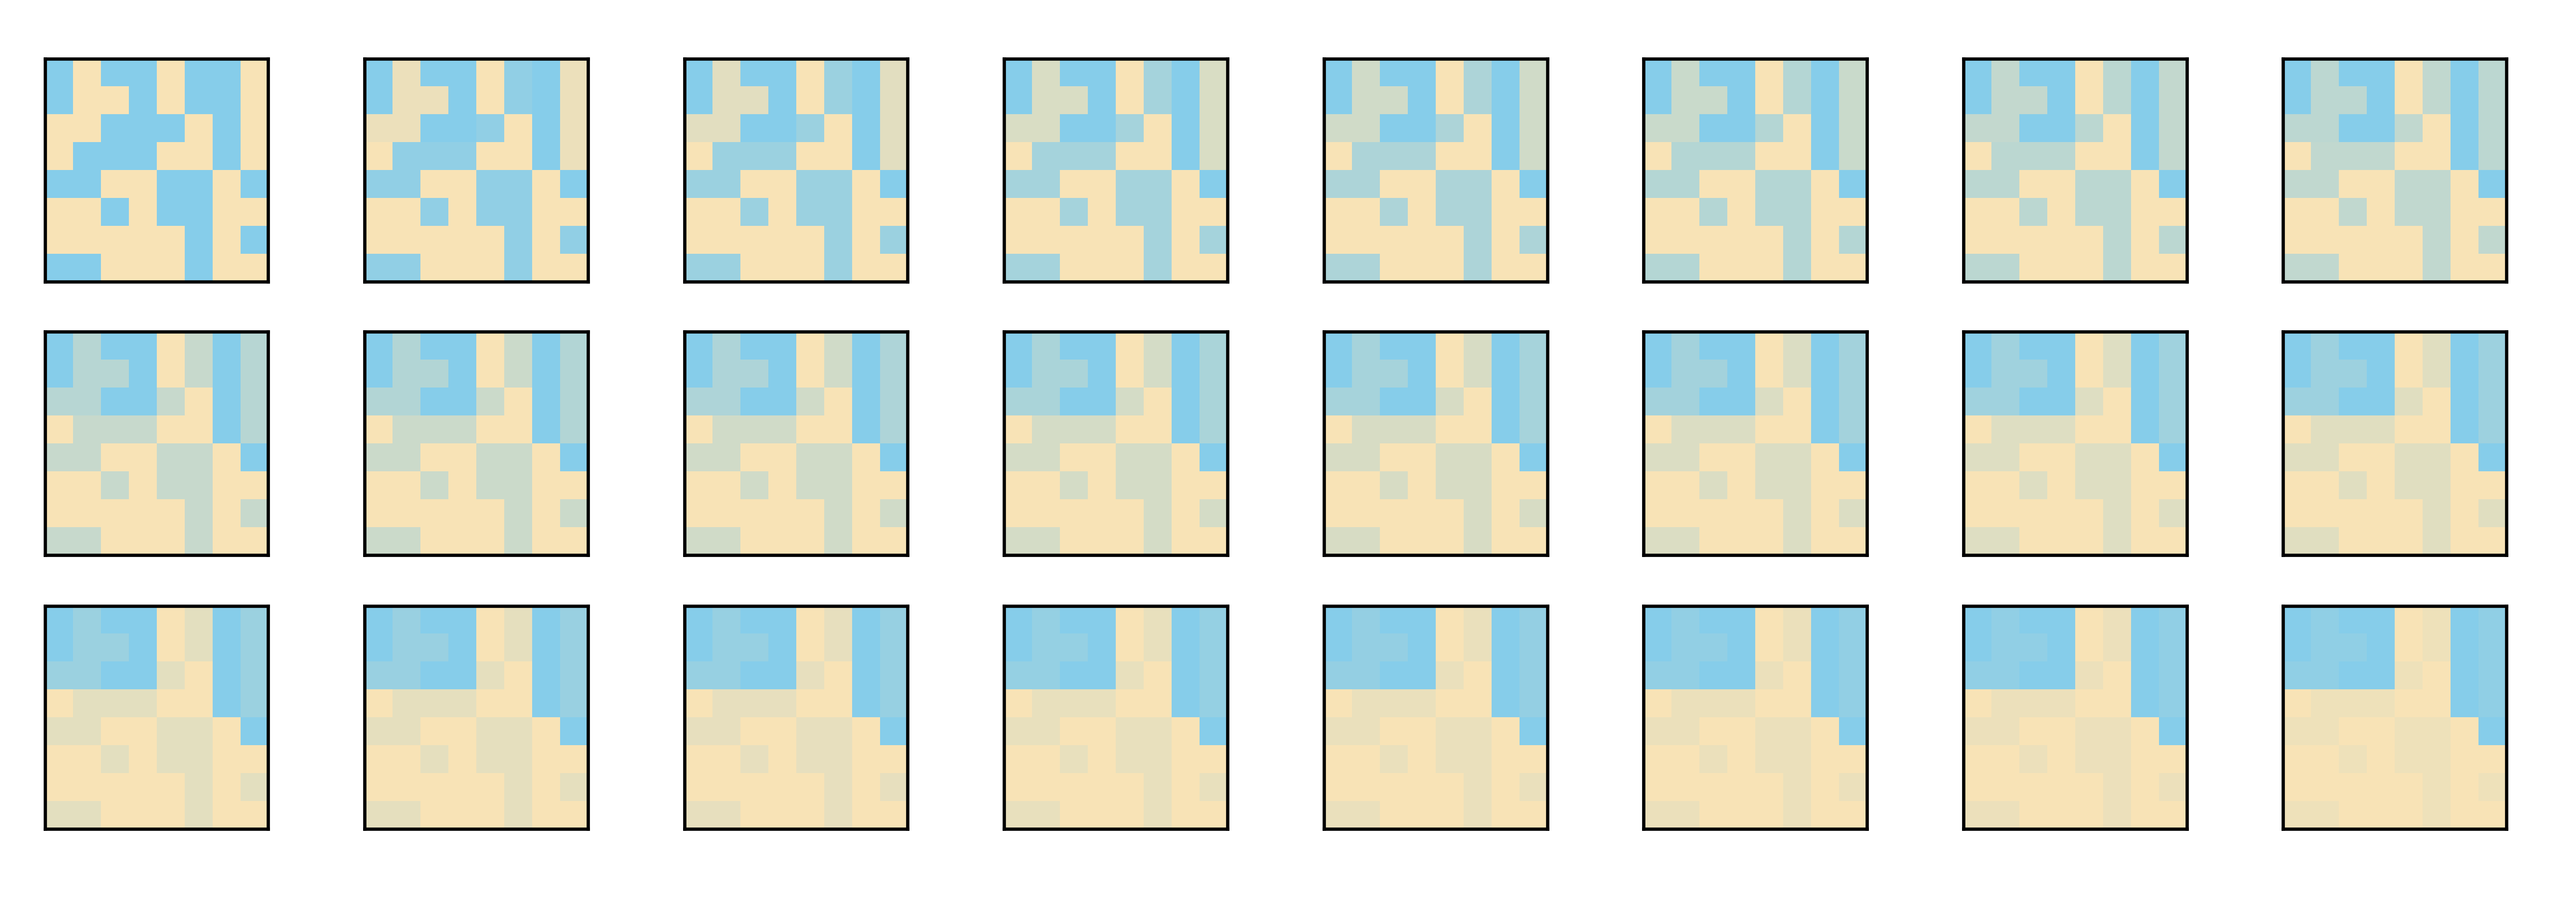
\includegraphics[width=.8\linewidth]{exercice5fig10.2.png}
\caption[spt]{See Figure \ref{fig:fig9}}\label{fig:fig10}
\end{figure}

Similarly, we can set the weights to store several patterns as follows:
\begin{equation}\label{eq:10}
  W=\frac{1}{N}\sum\mathbf{p}_i\mathbf{p}_i^T
\end{equation}
\indent And the networks stabilizes at the following patterns: $p,q, -p, -q$ (Figure \ref{fig:pat}).

\begin{figure}[H]
\centering
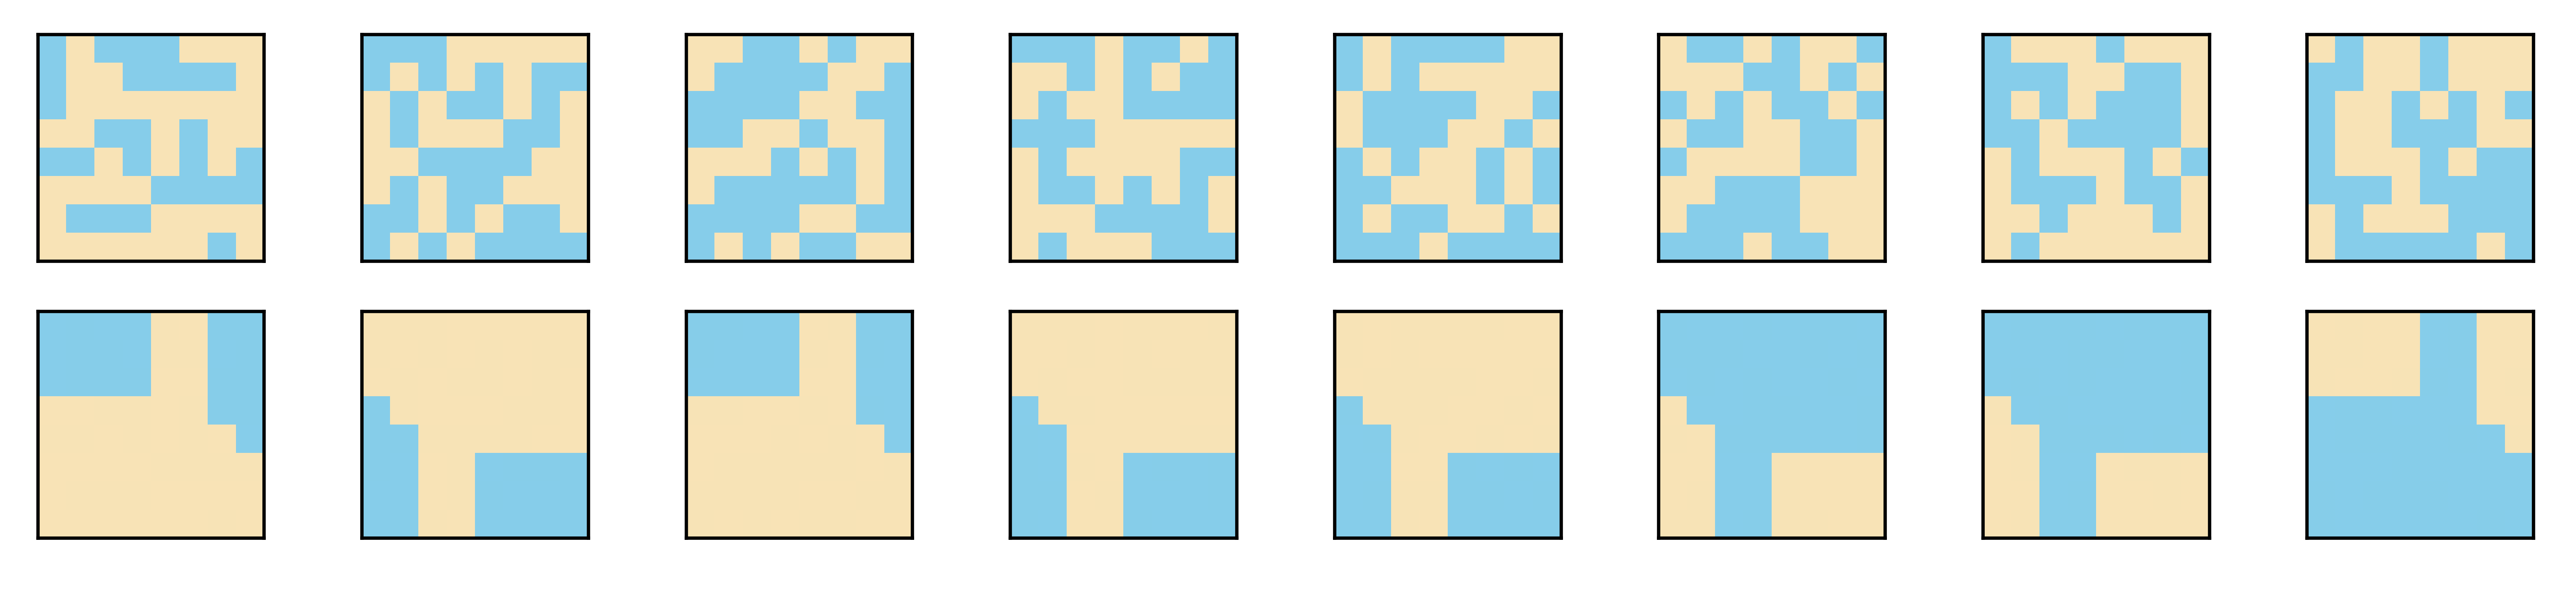
\includegraphics[width=.8\linewidth]{exercice5fig11.png}
\caption[spt]{Up row: random patterns fed into the system. Low row: pattern after 50 iterations of the Euler approximation for the network dynamics.}\label{fig:pat}
\end{figure}

\indent We might now ask ourselves how good is this neural network at recognizing altered patterns; as for instance our brain is able to rebuild half-erased letters on paper. If we change a few cells, it manages to bet back to the original rapidely, up to around 20 altered cells, where the result is less obvious and less frequently the original pattern (Figure \ref{fig:fig11} and \ref{fig:fig12})


\begin{figure}[H]
\centering
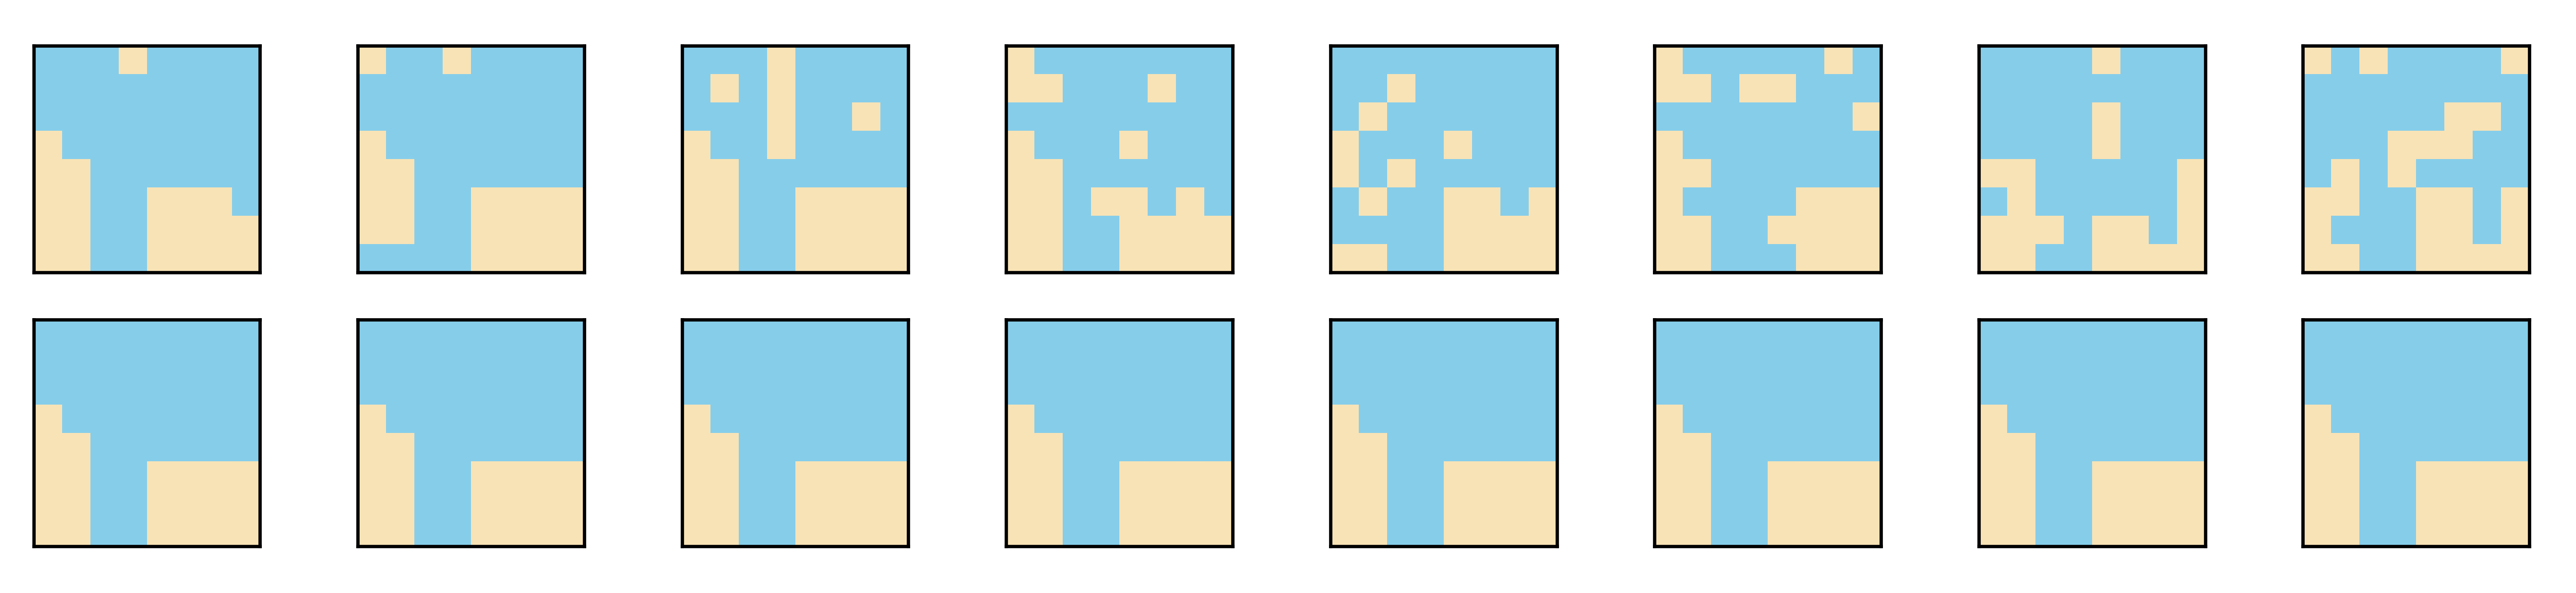
\includegraphics[width=.8\linewidth]{exercice5fig12.png}
\caption[spt]{Up row: altered $-q$ patterns fed into the system, from 2 to 16 cells changed. Low row: pattern after 50 iterations of the Euler approximation for the network dynamics.}\label{fig:fig11}
\end{figure}

\begin{figure}[H]
\centering
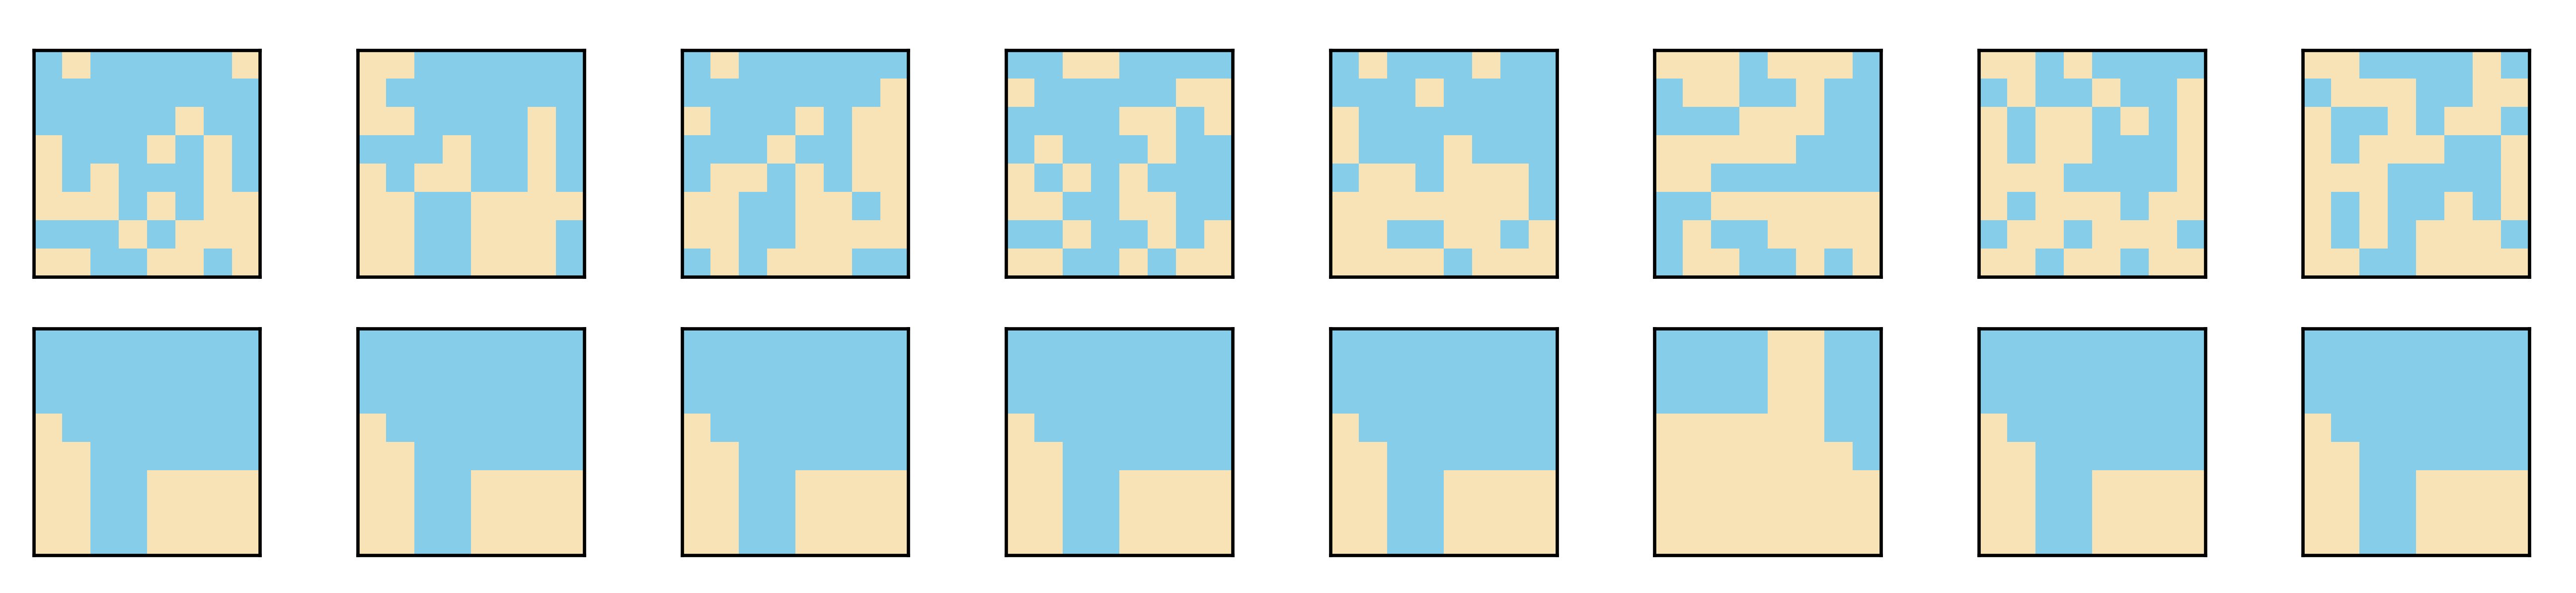
\includegraphics[width=.8\linewidth]{exercice5fig13.png}
\caption[spt]{See Figure \ref{fig:fig11}, from 18 to 32 cells changed.}\label{fig:fig12}
\end{figure}

Moreover, we can consider the same activation function as before (Section \ref{autapse}), and the network `pattern' could in that case represent the neurons firing rate. Or, the other way around, we can wonder if a real neural network with those properties could efficiently maintain a representation in working memory in this manner. Figure \ref{fig:fig13} shows such a simulation, and this yields some puzzling results. First, the networks converge more rapidly, and the cells firing rates tend to either 0 or 100. More unexpected, this activation function makes the network only yield $-p, -q, and -(p+q)$ patterns. The negative patterns are probably due to the combined firing rate having a specific equilibrium for such a function, and the combined pattern to the symetry of $p$ and $q$. This shows how important the choice of parameters is in modelling, especially if one wants to have an accurate biophysical description of neural networks.

\begin{figure}[H]
\centering
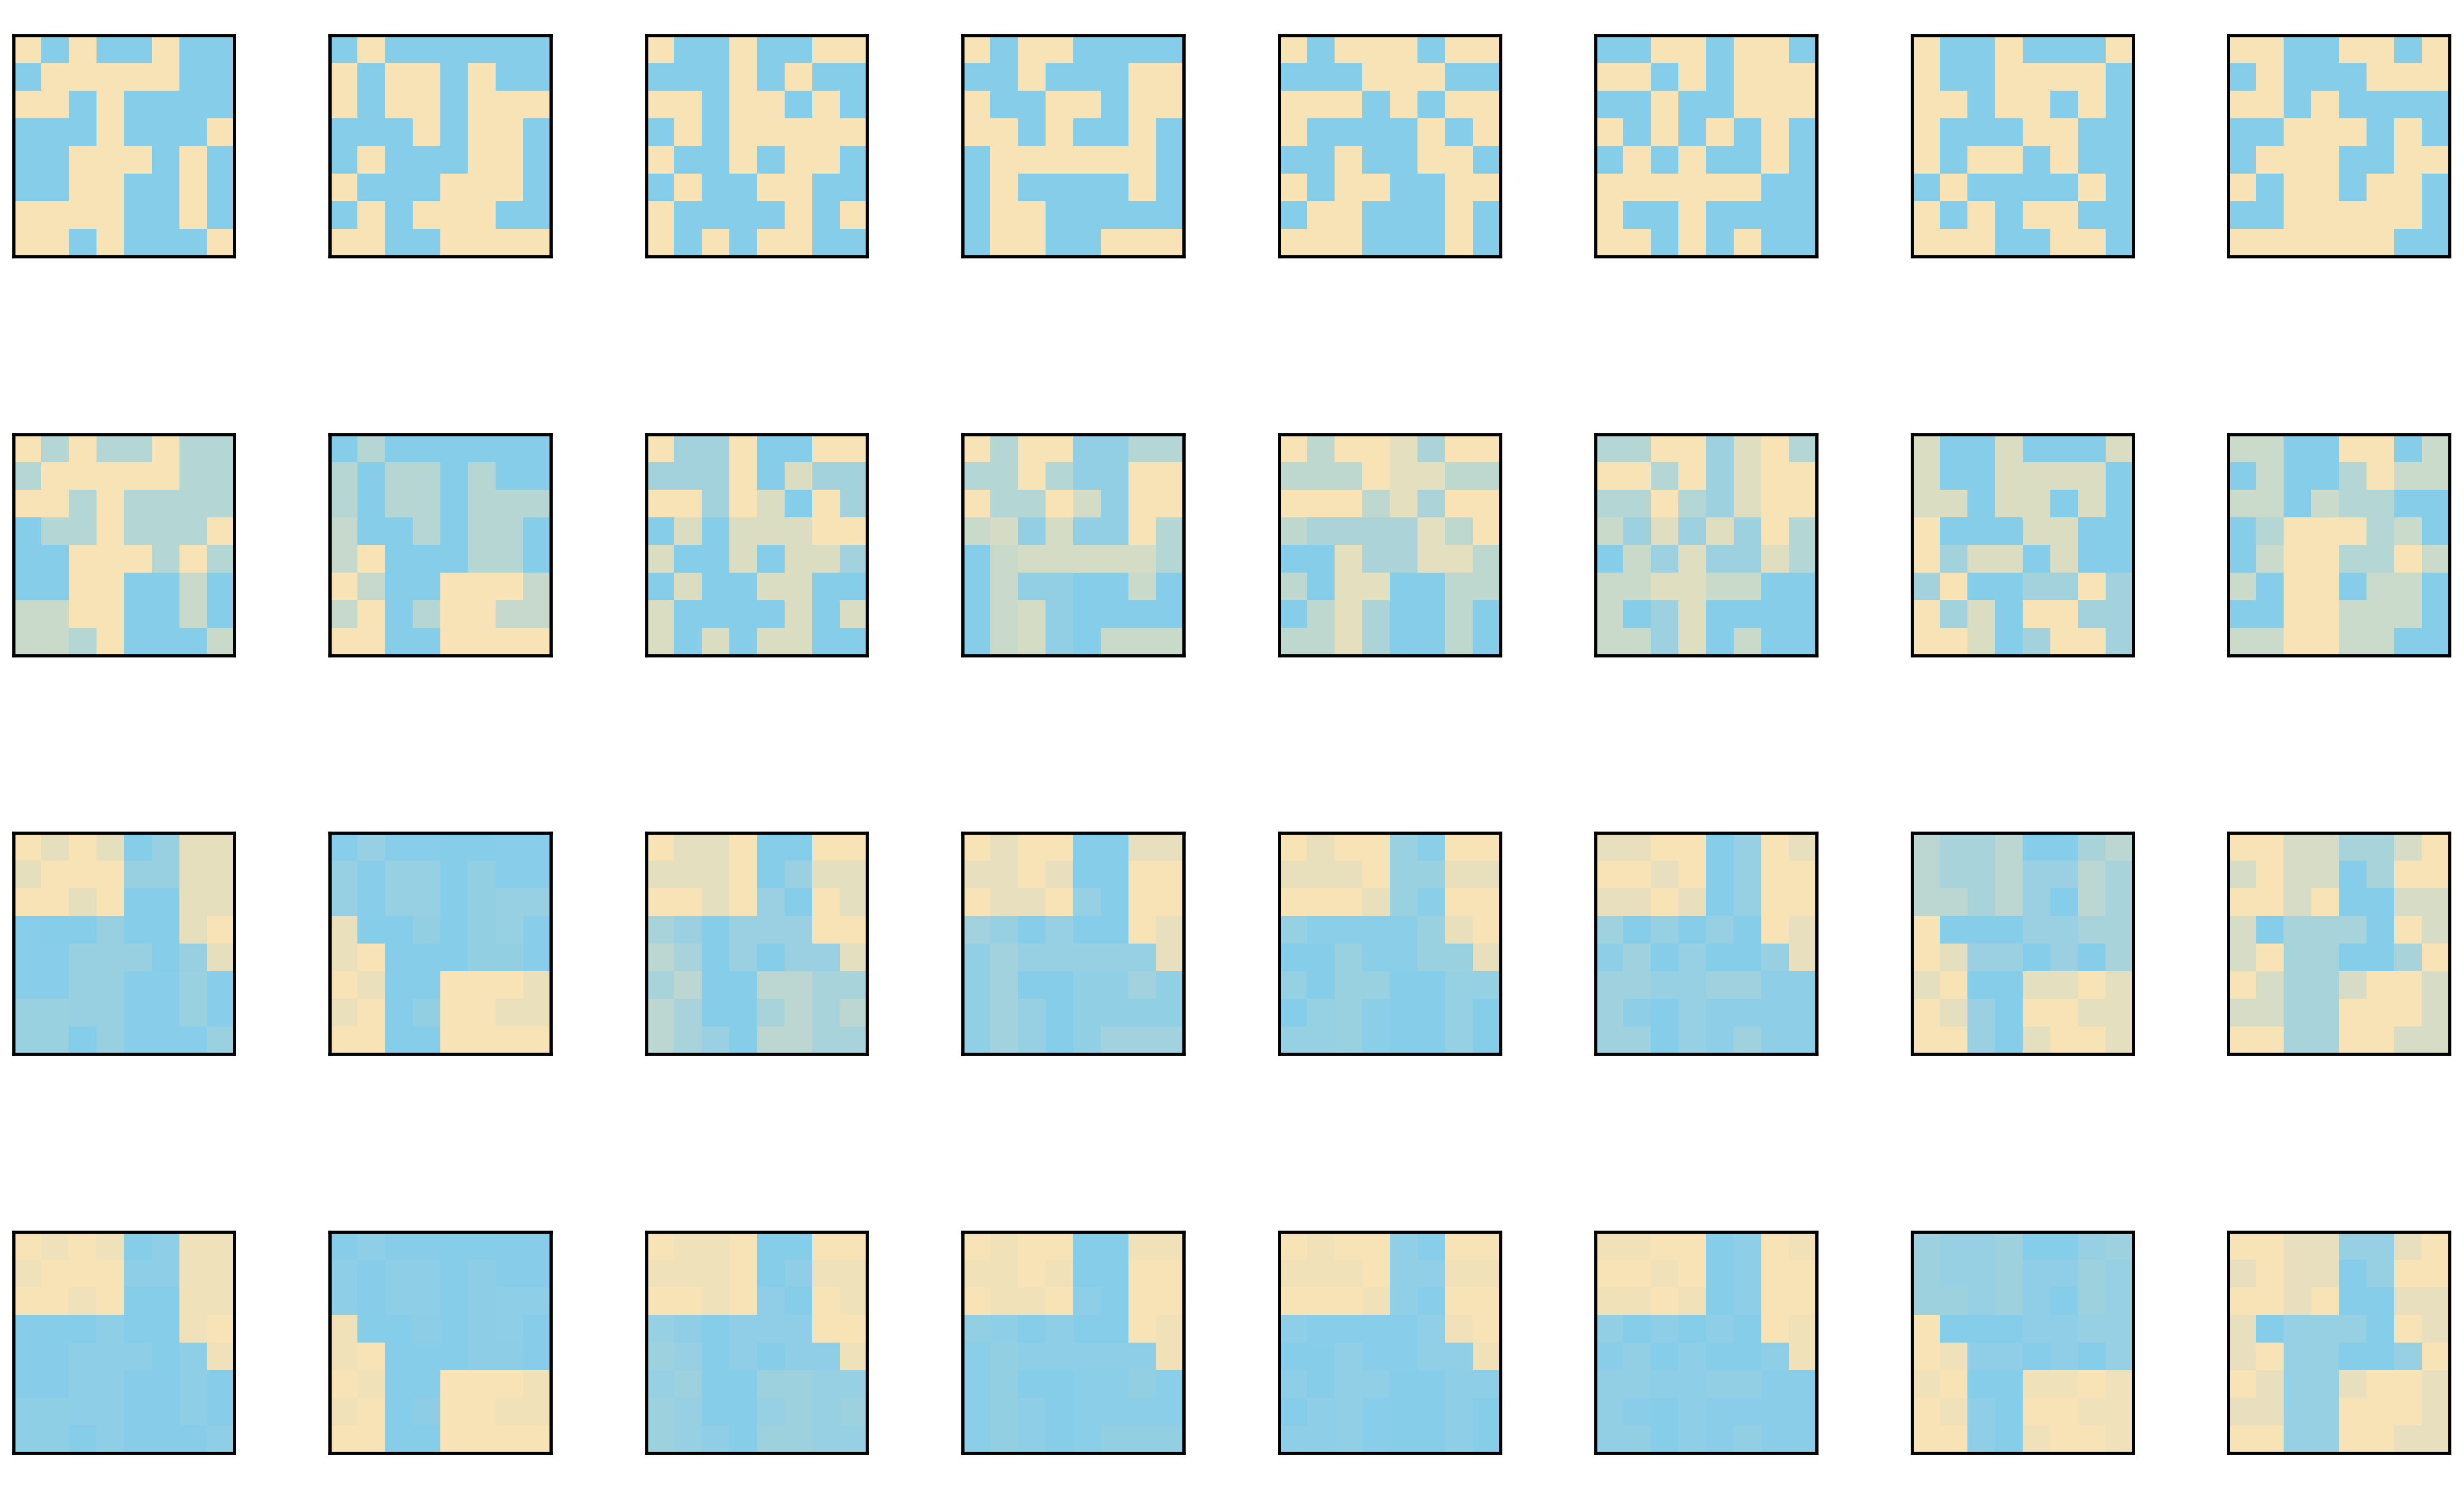
\includegraphics[width=.8\linewidth]{exercice5fig14.png}
\caption[spt]{Up row: random patterns fed into the system. Low row: pattern after 1,2 and 3 Euler approximations for the network dynamics.}\label{fig:fig13}
\end{figure}

Such networks have obvious limitations in the number of patterns they can store, but are still pretty efficient. Hertz et al. 1991 showed the recall accuracy was 0.138: 138 patterns can be stored for 1000 cells. However, other methods to fix the weights beforehand or through learning can yield higher performances.

\section{Conclusion}
\indent \indent In the previous sections, we saw that modelling a neural network isn't so complpicated. It is possible to model a neural network as a system of differential equation, and from there it is possible to study its dynamics with the dynamical systems' approach.
Moreover, this method allows to better understand the implications of different parameters. For instance, the combination of inhibitory synapses (and a sigmoidal activation function) will make neurons `compete` when there is an input current, until only one is active. Depending on the problem at hand, some aspects of the models can be simplified, like the spiking mechanism of a neuron that can be approximated by its firing rate, which is actually easier to interpret. \\
\indent Moreover, such networks have applications outside of neuroscience. For instance, section \ref{hopfield} showed a simple network was able to recognize patterns. This can be used optical character recognition, face recognition, classification of database images... In such case, biophysical accuracy is not a concern, only performance is; whereas neuroscientific approaches try to find what are the likely implementations of cognitive processes, and what neural network properties are important for the complex computations underlying them.

\end{document}
